\documentclass[preprint2]{aastex62}
\newcommand{\vdag}{(v)^\dagger}
\newcommand\aastex{AAS\TeX}
\newcommand\latex{La\TeX}

\usepackage{amsmath}
\usepackage{cancel}
\usepackage{float}

\shorttitle{Updated Opacities for DSEP}
\shortauthors{Boudreaux et al.}
% \watermark{DRAFT}
% \graphicspath{{./}{figures/}{src/figures}}

\begin{document}

\title{Updated High-Temperature Opacities for The Dartmouth Stellar Evolution
Program and their Effect on the Jao Gap Location}

\correspondingauthor{Thomas M. Boudreaux}
\email{thomas.m.boudreaux.gr@dartmouth.edu,\\thomas@boudreauxmail.com}

\author[0000-0002-2600-7513]{Thomas M. Boudreaux}
\affiliation{Department of Physics and Astronomy, Dartmouth College, Hanover, NH 03755, USA}

\author[0000-0003-3096-4161]{Brian C. Chaboyer}
\affiliation{Department of Physics and Astronomy, Dartmouth College, Hanover, NH 03755, USA}

\received{9/20/2022}
\revised{12/12/2022}
\revised{1/23/2023}
\accepted{1/24/2023}
% \submitjournal{ApJ}


\begin{abstract}

	The Jao Gap, a 17 percent decrease in stellar density at M$_{G} \sim$ 10
	identified in both Gaia DR2 and EDR3 data, presents a new method to probe
	the interior structure of stars near the fully convective transition mass.
	The Gap is believed to originate from convective kissing instability
	wherein asymmetric production of $^{3}$He causes the core convective zone
	of a star to periodically expand and contract and consequently the stars’
	luminosity to vary. Modeling of the Gap has revealed a sensitivity in its
	magnitude to a population’s metallicity primarily through opacity. Thus
	far, models of the Jao Gap have relied on OPAL high-temperature radiative
	opacities. Here we present updated synthetic population models tracing the
	Gap location modeled with the Dartmouth stellar evolution code using the
	OPLIB high-temperature radiative opacities. Use of these updated opacities
	changes the predicted location of the Jao Gap by $\sim$0.05 mag as compared
	to models which use the OPAL opacities. This difference is likeley too
	small to be detectable in empirical data.

\end{abstract}

\keywords{Stellar Evolution (1599) --- Stellar Evolutionary Models (2046)}

\section{Introduction}\label{sec:Intro}
Globular clusters (GCs) are among the oldest observable objects in the universe
\citep{Pen11}. They are characterized by high densities with typical half-light
radii of $\le$10 pc \citep{Vanderburg2010}, and typical masses ranging from
$10^{4}$--$10^{5}$ M$_{\odot}$ \citep{Bro06} --- though some GCs are
significantly larger than these typical values \citep[e.g. $\omega$ Cen,
][]{Richer1991}. GCs provide a unique way to probe stellar evolution
\citep{Bau03}, galaxy formation models \citep{Boy18,Kra05}, and dark matter
halo structure \citep{Hud18}.

The traditional view of Globular Clusters was that they consisted of a single
stellar population (SSP, in some publications this is referred to as a Simple
Stellar Population). This view was supported by spectroscopically uniform heavy
element abundances \citep{Carretta2010, Bastian2018} across most clusters (M54
and $\omega$Cen are notable exceptions, see \citet{Marino2015} for further
details), and the lack of evidence for multiple stellar populations (MPs) in
past color-magnitude diagrams of GCs \citep[i.e.][]{Sandage1953, Alcaino1975}.
However, over the last 40 years non-trivial star-to-star light-element
abundance variations have been observed \citep[i.e.][]{Smith1987} and, in the
last two decades, it has been definitively shown that most if not all Milky Way
GCs have MPs \citep{Gratton2004, Gratton2012, Piotto2015}. The lack of
photometric evidence for MPs prior to the 2000, can be attributed to the more
narrow color bands available, until very recently, to ground based photometric
surveys \citep{Milone2017}.

The prevalence of multiple populations in GCs is so distinct that the proposed
definitions for what constitutes a globular cluster now often center the
existence of MPs \citep[e.g.][]{Carretta2010}. Whereas, people have have often
tried to categorized objects as GCs through relations between half-light
radius, density, and surface brightness profile, in fact many objects which are
generally thought of as GCs don't cleanly fit into these cuts
\citep{Peebles1968, Brown1991, Brown1995, Bekki2002}. Consequently,
\citet{Carretta2010} proposed a definition of GC based on observed chemical
inhomogeneities in their stellar populations. The modern understanding of GCs
then is not simply one of a dense cluster of stars that may have chemical
inhomogeneities and multiple populations; rather, it is one where those
chemical inhomogeneities and multiple populations themselves are the defining
element of a GC.

All Milky Way globular clusters studied in detail show populations enriched in
He, N, and Na while also being deplete in O and C
\citep{Piotto2015,Bastian2018}. {\bf Further, studies of Magellenic Cloud
massive clusters have shown that these light element abundance variations exist
in clusters as young as $\sim 2$ Gyr but not in younger clusters
\citep{Martocchia2019} while there is also evidence of nitrogen variability in
the $\sim 1.5$ Gyr old cluster NGC 1783 \citep{Cadelano2022}}.  These light
element abundance patterns also are not strongly correlated with variations in
heavy element abundance, resulting in spectroscopically uniform Fe abundances
between populations \citep[{\bf though recent work indicates that there may be
[Fe/H] variations within the first population, e.g.}][]{Legnardi2022,
Lardo2022} . Further, high-resolution spectral studies reveal anti-correlations
between N-C abundances, Na-O abundances, and potentially Al-Mg
\citep{Sneden1992, Gratton2012}. Typical stellar fusion reactions can deplete
core oxygen; however, the observed abundances of Na, Al, and Mg cannot be
explained by the CNO cycle \citep{Prantzos2007}. Consequently, globular cluster
populations must be formed by some novel means.

Formation channels for these multiple populations remain a point of debate
among astronomers. Most proposed formation channels consist of some older,
more massive, population of stars polluting the pristine cluster media before a
second population forms, now enriched in heavier elements which they themselves could
not have generated \citep[for a detailed review see ][]{Gratton2012}. The four
primary candidates for these polluters are asymptotic giant branch stars
\citep[AGBs,][]{Ventura2001,DErcole2010}, fast rotating massive stars
\citep[FRMSs,][]{Decressin2007}, super massive stars
\citep[SMSs,][]{Denissenkov2014}, and massive interacting binaries
\citep[MIBs,][]{deMink2009, Bastian2018}. 

Hot hydrogen burning (i.e. proton capture), material transport to the surface, and
material ejection into the intra-cluster media are features of each of these
models and consequently they can all be made to {\it qualitatively} agree with
the observed elemental abundances. However, none of the standard models can
currently account for all specific abundances \citep{Gratton2012}. AGB and FRMS
models are the most promising; however, both models have difficulty reproducing
severe O depletion \citep{Ventura2009,Decressin2007}. Moreover, AGB and FRMS
models require significant mass loss ($\sim 90\%$) between cluster formation
and the current epoch --- implying that a significant fraction of halo stars
formed in GCs \citep{Renzini2008,DErcole2008,Bastian2015}.

In addition to the light-element anti-correlations observed, it is also known
that second populations are significantly enhanced in Helium
\citep{Piotto2007, Piotto2015, Latour2019}. Depending on the cluster, helium
mass fractions as high as $Y=0.4$ have been inferred \citep[e.g][]{Milone2015}.
However, due to both the relatively high and tight temperature range of partial
ionization for He and the efficiency of gravitational settling in core helium
burning stars, the initial He abundance of globular cluster stars cannot be
observed; consequently, the evidence for enhanced He in GCs originates from
comparison of theoretical stellar isochrones to the observed
color-magnitude-diagrams of globular clusters. Therefore, a careful handling of
chemistry is essential when modeling with the aim of discriminating between
MPs; yet, only a very limited number of GCs have been studied with
chemically self-consistent (structure and atmosphere) isochrones
\citep[e.g.][NGC 6752]{Dotter2015}. 

NGC 2808 is the prototype globular cluster to host Multiple Populations.
Various studies since 2007 have identified that it may host anywhere from 2-5
stellar populations. These populations have been identified both
spectroscopically \citep[i.e.][]{Carretta2004, Carretta2006, Carretta2010,
Gratton2011, Carretta2015, Hong2021} and photometrically
\citep[i.e.][]{Piotto2007, Piotto2015, Milone2015, Milone2017, Pasquato2019}.
Note that recent work \citep{Valle2022} calls into question the statistical
significance of the detections of more than 2 populations in the spectroscopic
data. Here we present new, chemically self-consistent modeling of the
photometry of the two extreme populations of NGC 2808 identified by
\citet{Milone2015}, populations A and E. {\bf We do not consider populations B,
C, or D identified in \citet{Milone2015} as the purpose of this work is to
identify if chemically self-consistent modelling results in a statisically
signifigant deviation in the infered helium abundance when compared to non
chemically self-consistent models. Use of the two populations in the NGC 2808
with the highest identified difference between their helium populations is
sufficent for to answer this question.}  We use archival photometry from the
Hubble UV Globular Cluster Survey (HUGS) \citep{Piotto2015, Milone2017} in the
F275W and F814W passbands to characterize multiple populations in NGC 2808
\citep{Milone2015, Milone2015b} (This data is avalible at MAST: \href{https://archive.stsci.edu/doi/resolve/resolve.html?doi=10.17909/T9810F}{10.17909/T9810F}). Additionally, we present a
likelihood analysis of the photometric data of NGC 2808 to determine the number
of populations present in the cluster.




\section{The Underlying Physics of the Gap}\label{sec:JaoGap}
A theoretical explanation for the Jao Gap (Figure \ref{fig:JaoGap}) comes from
\citet{van2012}, who propose that in a star directly above the transition mass,
due to asymmetric production and destruction of $^{3}$He during the
proton-proton I chain (ppI), periodic luminosity variations can be induced.
This process is known as convective-kissing instability. Very shortly after the
zero-age main sequence such a star will briefly develop a radiative core;
however, as the core temperature exceeds $7\times 10^{6}$ K, enough energy will
be produced by the ppI chain that the core once again becomes convective. At
this point the star exists with both a convective core and envelope, in
addition to a thin, radiative layer separating the two. Subsequently,
asymmetries in ppI affect the evolution of the star's convective core.

While kissing instability has been the most widely adopted model to
explain the existence of the Jao Gap, slightly different mechanisms have also
been proposed. \citet{MacDonald2018} make use of a fully implicit stellar
evolution suite which treats convective mixing as a diffusive property.
\citeauthor{MacDonald2018} treat convective mixing this way in order to account
for a core deuterium concentration gradient proposed by \citet{Baraffe1997}.
Under this treatment the instability results only in a single mixing event ---
as opposed to periodic mixing events. Single mixing events may be more in line with
observations (see section \ref{sec:results} for more details on how periodic
mixing can effect a synthetic population) where there is only well documented
evidence of a single gap. However, recent work by \citet{Jao2021} which
identify an second under density of stars below the canonical gap, does leave
the door open for the periodic mixing events.

\begin{figure}
	\centering
	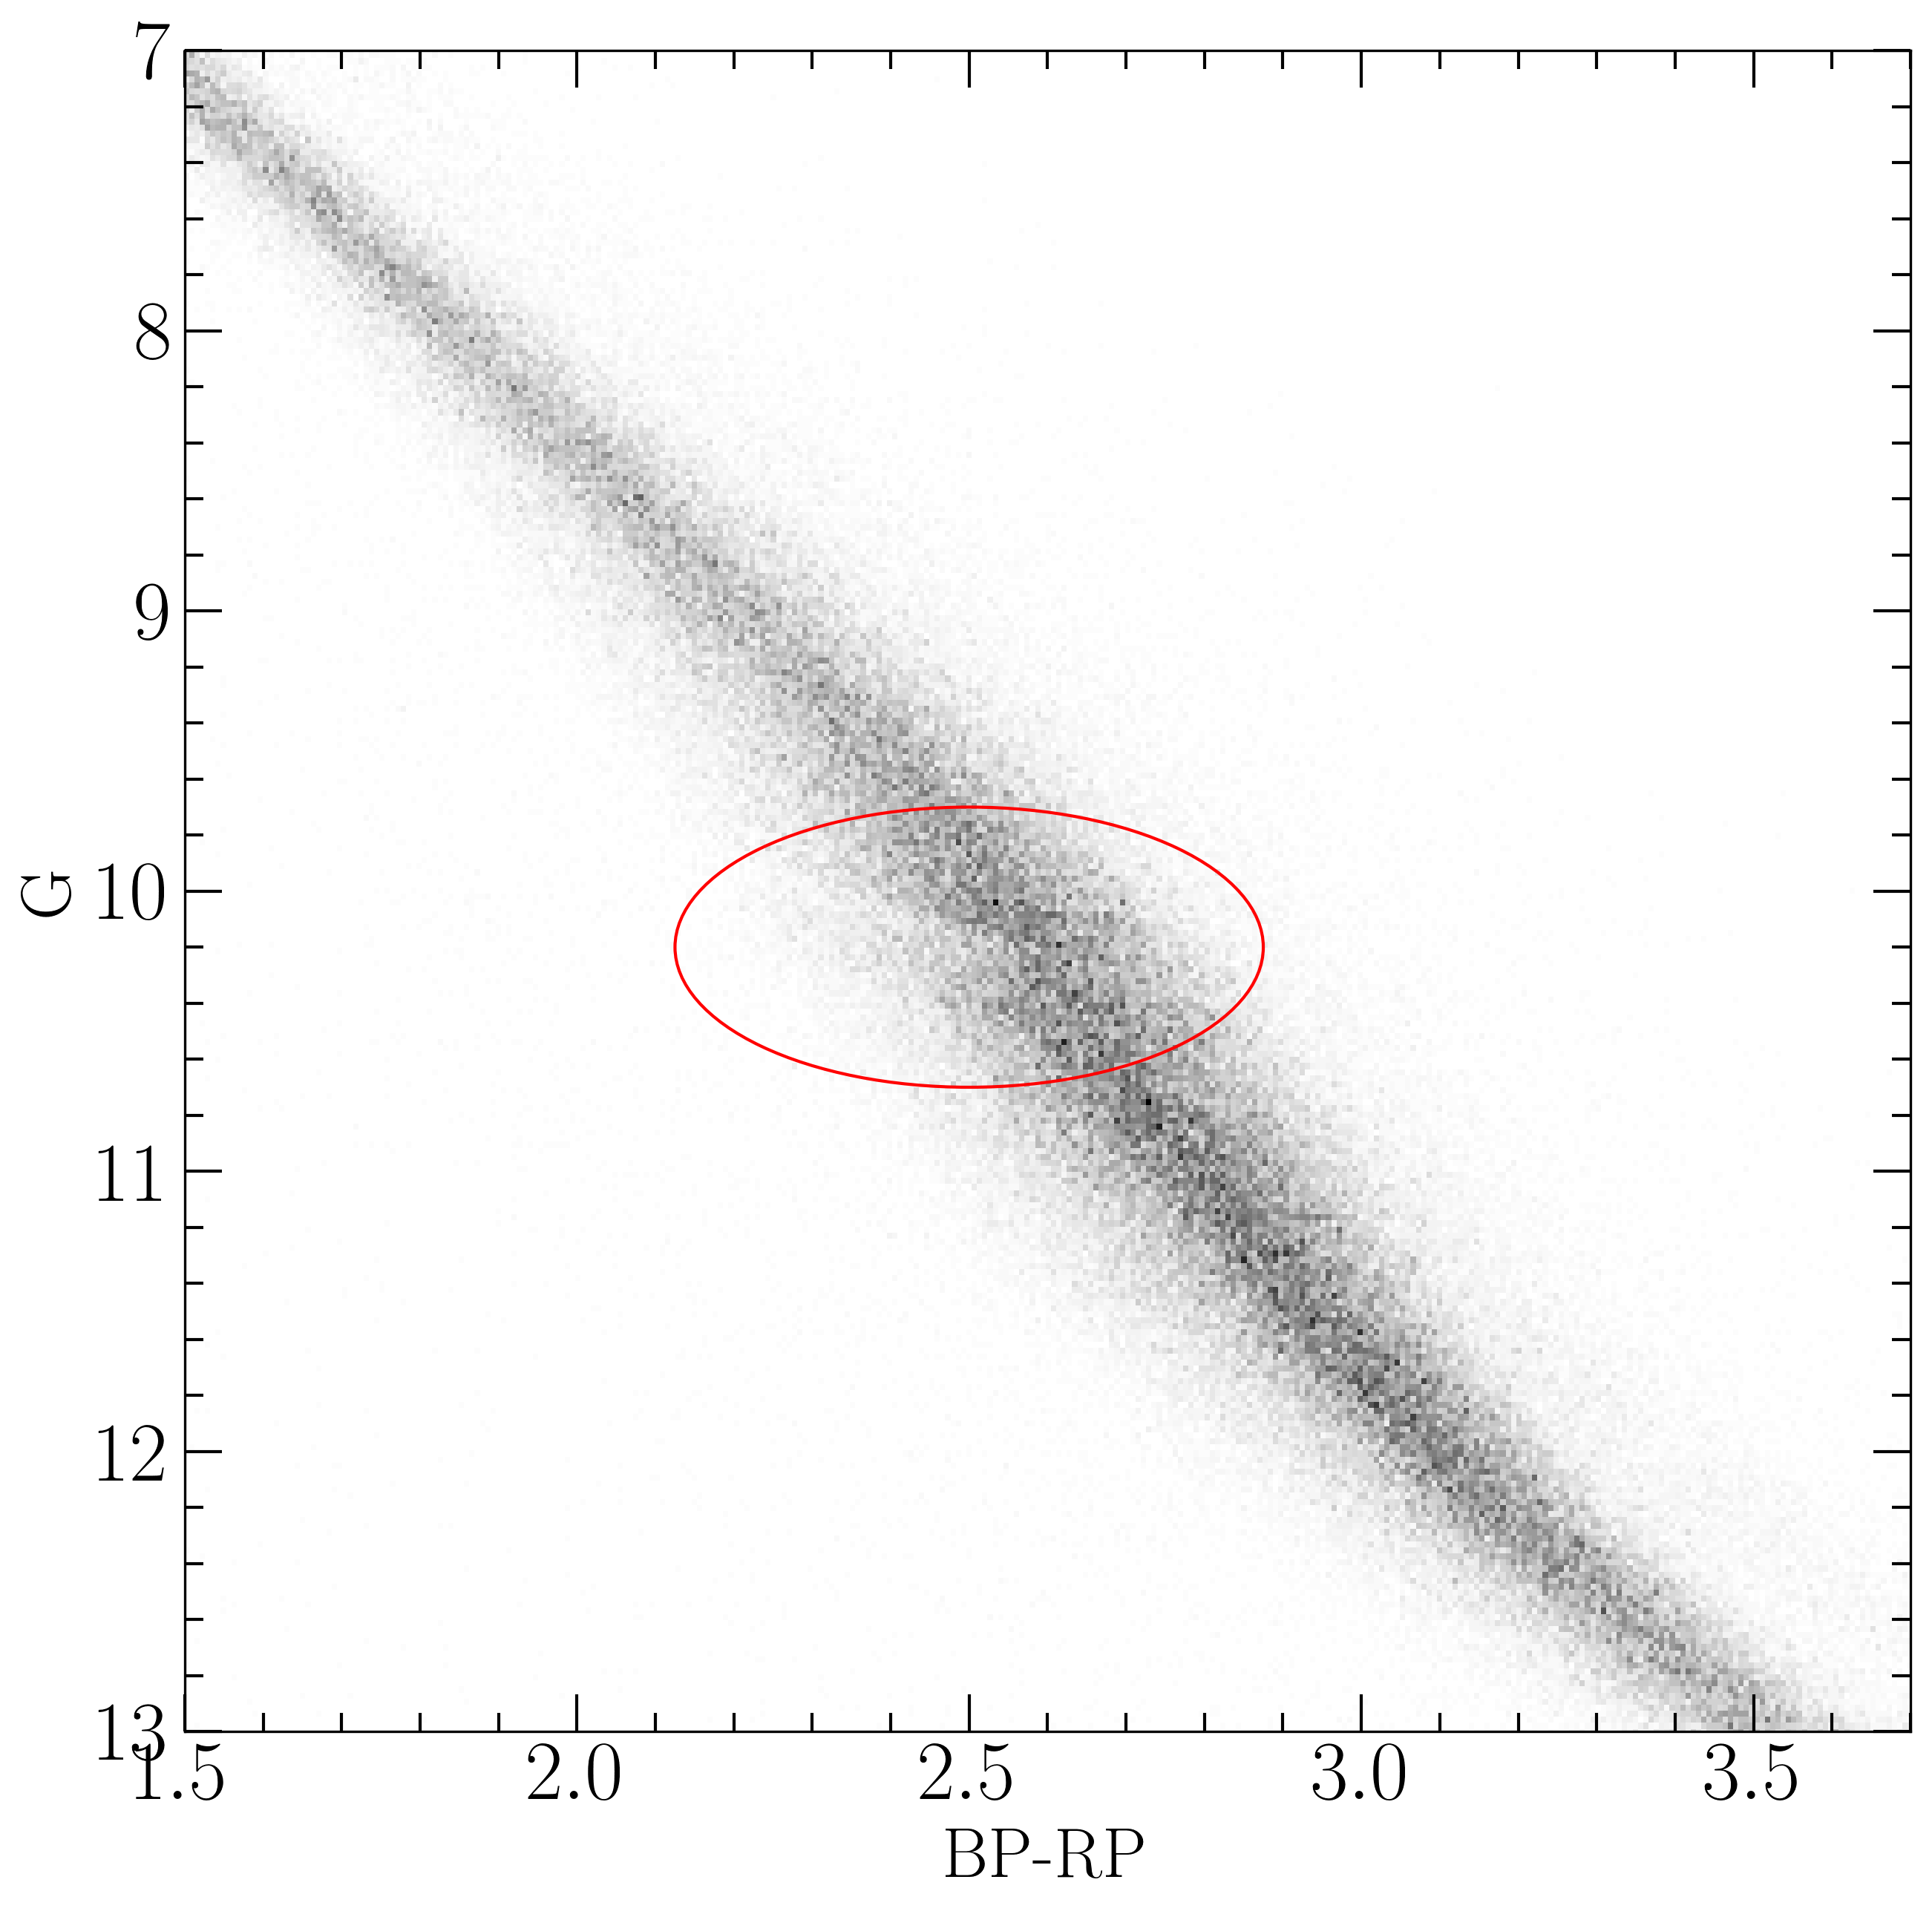
\includegraphics[width=0.85\textwidth]{figures/jaoOpacity/JaoGapEDR3.png}
	\caption{The Jao Gap (circled) seen in the Gaia Catalogue of Nearby Stars \citep{GaiaCollaboration2021}.}
	\label{fig:JaoGap}
\end{figure}

The proton-proton I chain constitutes three reactions 
\begin{enumerate} 
	\item $p + p \longrightarrow d + e^{+} + \nu_{e}$
	\item $p + d \longrightarrow \ ^{3}\text{He} + \gamma$
	\item $^{3}\text{He} + ^{3}\text{He} \longrightarrow \ ^{3}\text{He} + 2p$ 
\end{enumerate} 
Initially, reaction 3 of ppI consumes $^{3}$He at a slower rate than it is
produced by reaction 2 and as a result, the core $^{3}$He abundance and
consequently the rate of reaction 3, increases with time. The core convective
zone expands as more of the star becomes unstable to convection. This expansion
continues until the core connects with the convective envelope. At this point
convective mixing can transport material throughout the entire star and the
high concentration of $^{3}$He rapidly diffuses outward, away from the core,
decreasing energy generation as reaction 3 slows down. Ultimately, this leads
to the convective region around the core pulling back away from the convective
envelope, leaving in place the radiative transition zone, at which point
$^{3}$He concentrations grow in the core until it once again expands to meet
the envelope.  These periodic mixing events will continue until $^{3}$He
concentrations throughout the star reach an equilibrium ultimately resulting in
a fully convective star. Figure \ref{fig:Kippenhan1} traces the evolution of a
characteristic star within the Jao Gap's mass range.

\begin{figure*}
	\centering
	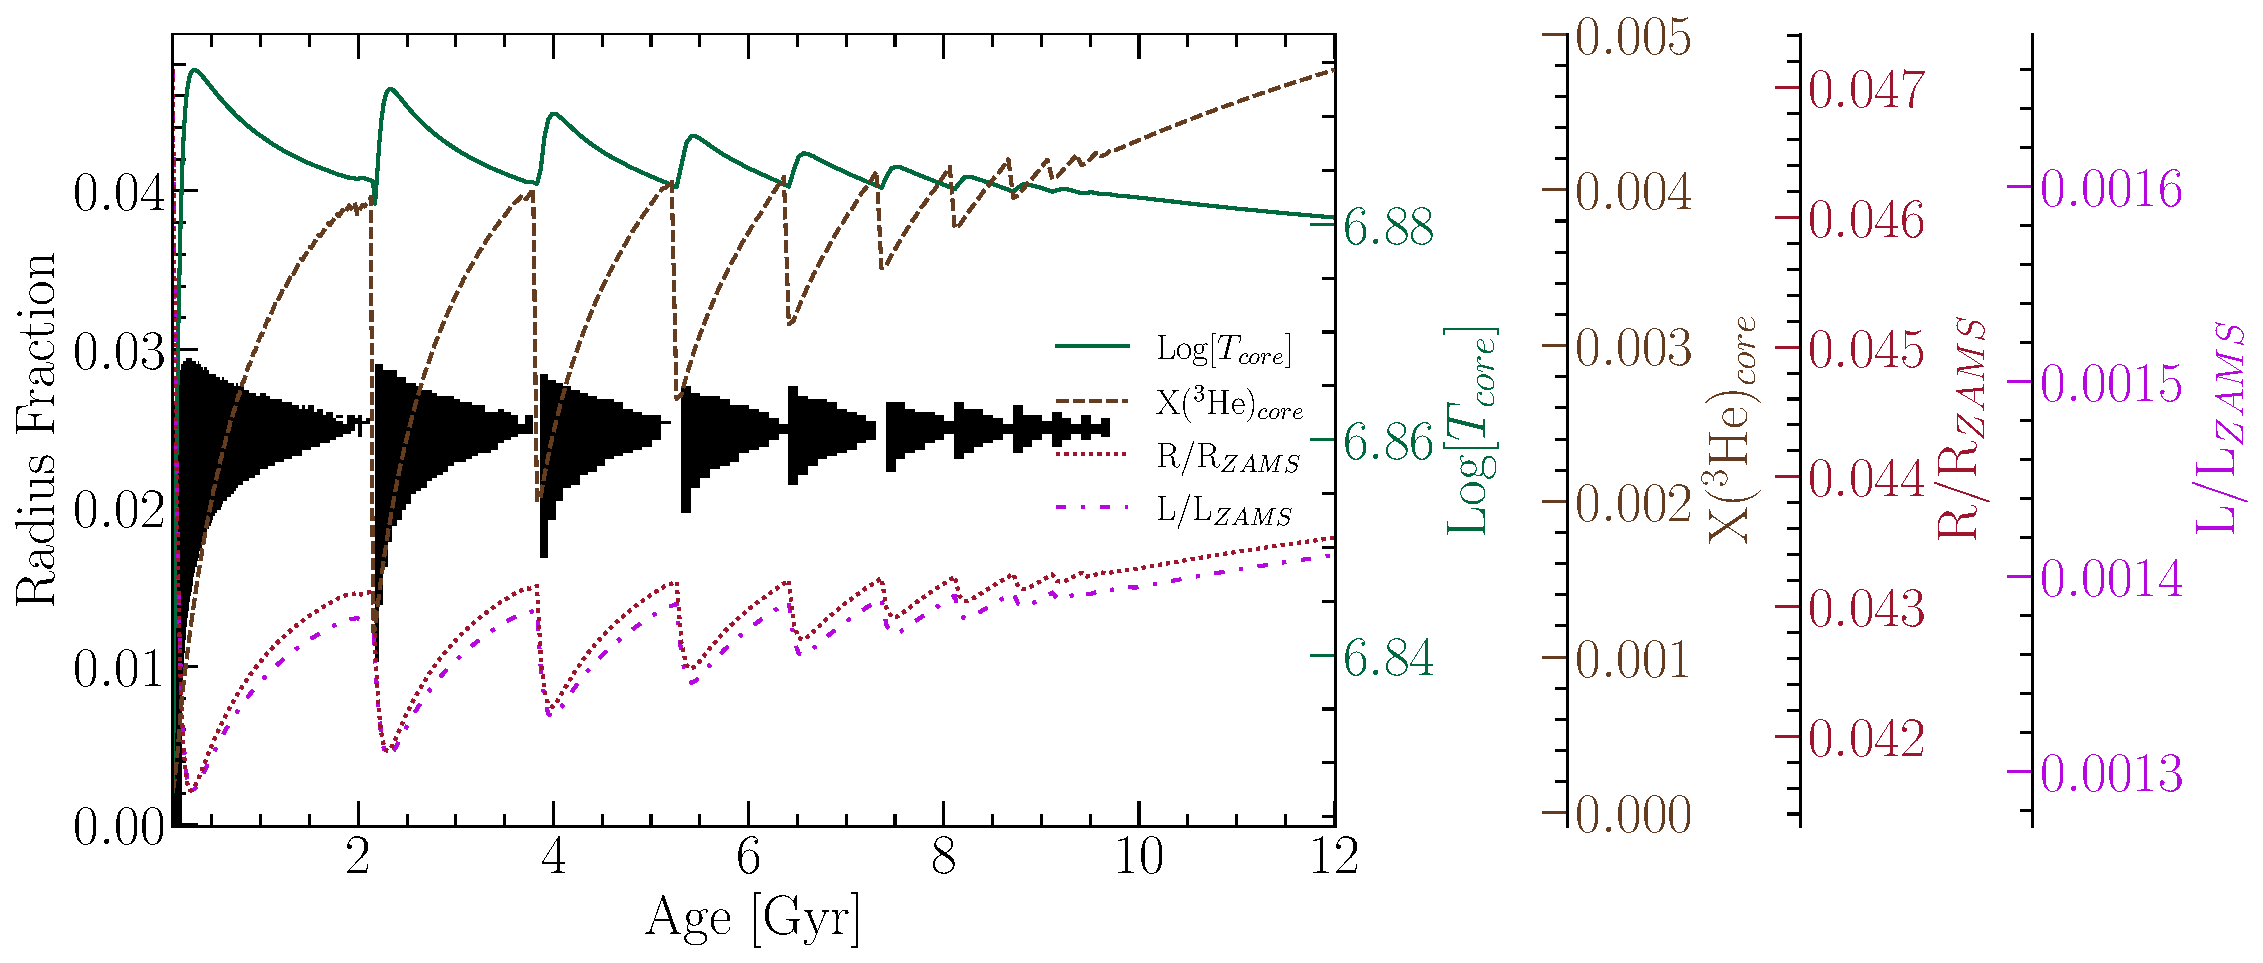
\includegraphics[width=0.95\textwidth]{figures/jaoOpacity/Kippenhan.pdf}
	\caption{Diagram for a characteristic stellar model of 0.35625 $M_{\odot}$
	which is within the Jao Gap's mass range. The black shaded regions denote
	whether, at a particular model age, a radial shell within the model is
	radiative (with white meaning convective). The lines trace the models core
	temperature, core $^{3}$He mass fraction, fractional luminosity wrt. the
	zero age main sequence and fractional radius wrt. the zero age main
	sequence.}
	\label{fig:Kippenhan1}
\end{figure*}


\subsection{Efforts to Model the Gap}
Since the identification of the Gap, stellar modeling has been
conducted to better constrain its location, effects, and exact cause.
Both \citet{Mansfield2021} and \citet{Feiden2021} identify that the Gap's mass
location is correlated with model metallicity --- the mass-luminosity
discontinuity in lower metallicity models being at a commensurately lower mass.
\citet{Feiden2021} suggests this dependence is due to the steep relation of
the radiative temperature gradient, $\nabla_{rad}$, on temperature and, in turn,
on stellar mass.

\begin{align}\label{eqn:radGrad}
	\nabla_{rad} \propto \frac{L\kappa}{T^{4}}
\end{align}

As metallicity decreases so does opacity, which, by Equation \ref{eqn:radGrad},
dramatically lowers the temperature at which radiation will dominate energy
transport \citep{Chabrier1997}. Since main sequence stars are virialized the
core temperature is proportional to the core density and total mass. Therefore,
if the core temperature where convective-kissing instability is expected
decreases with metallicity, so too will the mass of stars which experience such
instabilities.

% \begin{align}\label{eqn:TMRelation}
% 	T_{c} \propto \rho_{c}M^{2}
% \end{align}

The strong opacity dependence of the Jao Gap begs the question: what is
the effect of different opacity calculations on Gap properties.
As we can see above, changing opacity should affect the Gap's location in the
mass-luminosity relation and therefore in a color-magnitude diagram. Moreover,
current models of the Gap have yet to locate it precisely in the CMD
\citep{Feiden2021} with an approximate 0.16 G-magnitude difference between the
observed and modeled Gaps. Opacity provides one, as yet unexplored, parameter
which has the potential to resolve these discrepancies.


\section{Updated Opacities}\label{sec:opac}
% Radiative opacity is fundamental to stellar structure, it determines how much
% incident radiation is absorbed or scattered. Moreover, when a media is in
% thermodynamic equilibrium with the radiation field, that is when the temperature
% of the media and that of the radiation field is the same, the opacity may be
% used via Kirchhoff's law to find the emissivity of a material
% \citep{Huebner2014}. Local Thermodynamic Equilibrium (LTE) is a common state to
% find within a star and therefore stellar models have long relied on opacities
% calculated in LTE.
Multiple groups have released high-temperature opacities including, the Opacity
Project \citep[OP][]{Seaton1994}, Laurence Livermore National Labs OPAL opacity
tables \citep{Iglesias1996}, and Los Alamos National Labs OPLIB opacity tables
\citep{Colgan2016}. OPAL high-temperature radiative opacity tables in
particular are very widely used by current generation isochrone grids
\citep[e.g. Dartmouth, MIST, \& StarEvol, ][]{Dotter2008,Choi2016,Amard2019}.
OPLIB opacity tables \citep{Colgan2016} are not widely used but include the
most up-to-date plasma modeling.

While the overall effect on the CMD of using OPLIB compared to OPAL tables is
small, the strong theoretical opacity dependence of the Jao Gap raises the
potential for these small effects to measurably shift the Gap's location. We
update DSEP to use high temperature opacity tables based on measurements from
Los Alamos national Labs T-1 group \citep[OPLIB,][]{Colgan2016}. The OPLIB
tables are created with ATOMIC \citep{Magee2004,Hakel2006,Fontes2016}, a modern
LTE and non-LTE opacity and plasma modeling code. These updated tables were
initially created in order to incorporate the most up to date plasma
physics at the time \citep{Bahcall2005}. 

OPLIB tables include monochromatic Rosseland mean opacities --- composed from
bound-bound, bound-free, free-free, and scattering opacities --- for elements
hydrogen through zinc over temperatures 0.5eV to 100 keV (5802 K -- 1.16$\times
10 ^{9}$ K) and for mass densities from approximately $10^{-8}$ g cm$^{-3}$ up
to approximately $10^{4}$ g cm$^{-3}$ (though the exact mass density range
varies as a function of temperature). 

DSEP ramps the \citet{Ferguson2005} low temperature opacities to high
temperature opacities tables between $10^{4.3}$ K and $10^{4.5}$ K; therefore,
only differences between high-temperature opacity sources above $10^{4.3}$ K
can effect model evolution. When comparing OPAL and OPLIB opacity tables
(Figure \ref{fig:opacComp}) we find OPLIB opacities are systematically lower
than OPAL opacities for temperatures above $10^{5}$ K. Between $10^{4.3}$ and
$10^{5} K$ OPLIB opacities are larger than OPAL opacities. These generally
lower opacities will decrease the radiative temperature gradient throughout
much of the radius of a model.

\begin{figure}
	\centering
	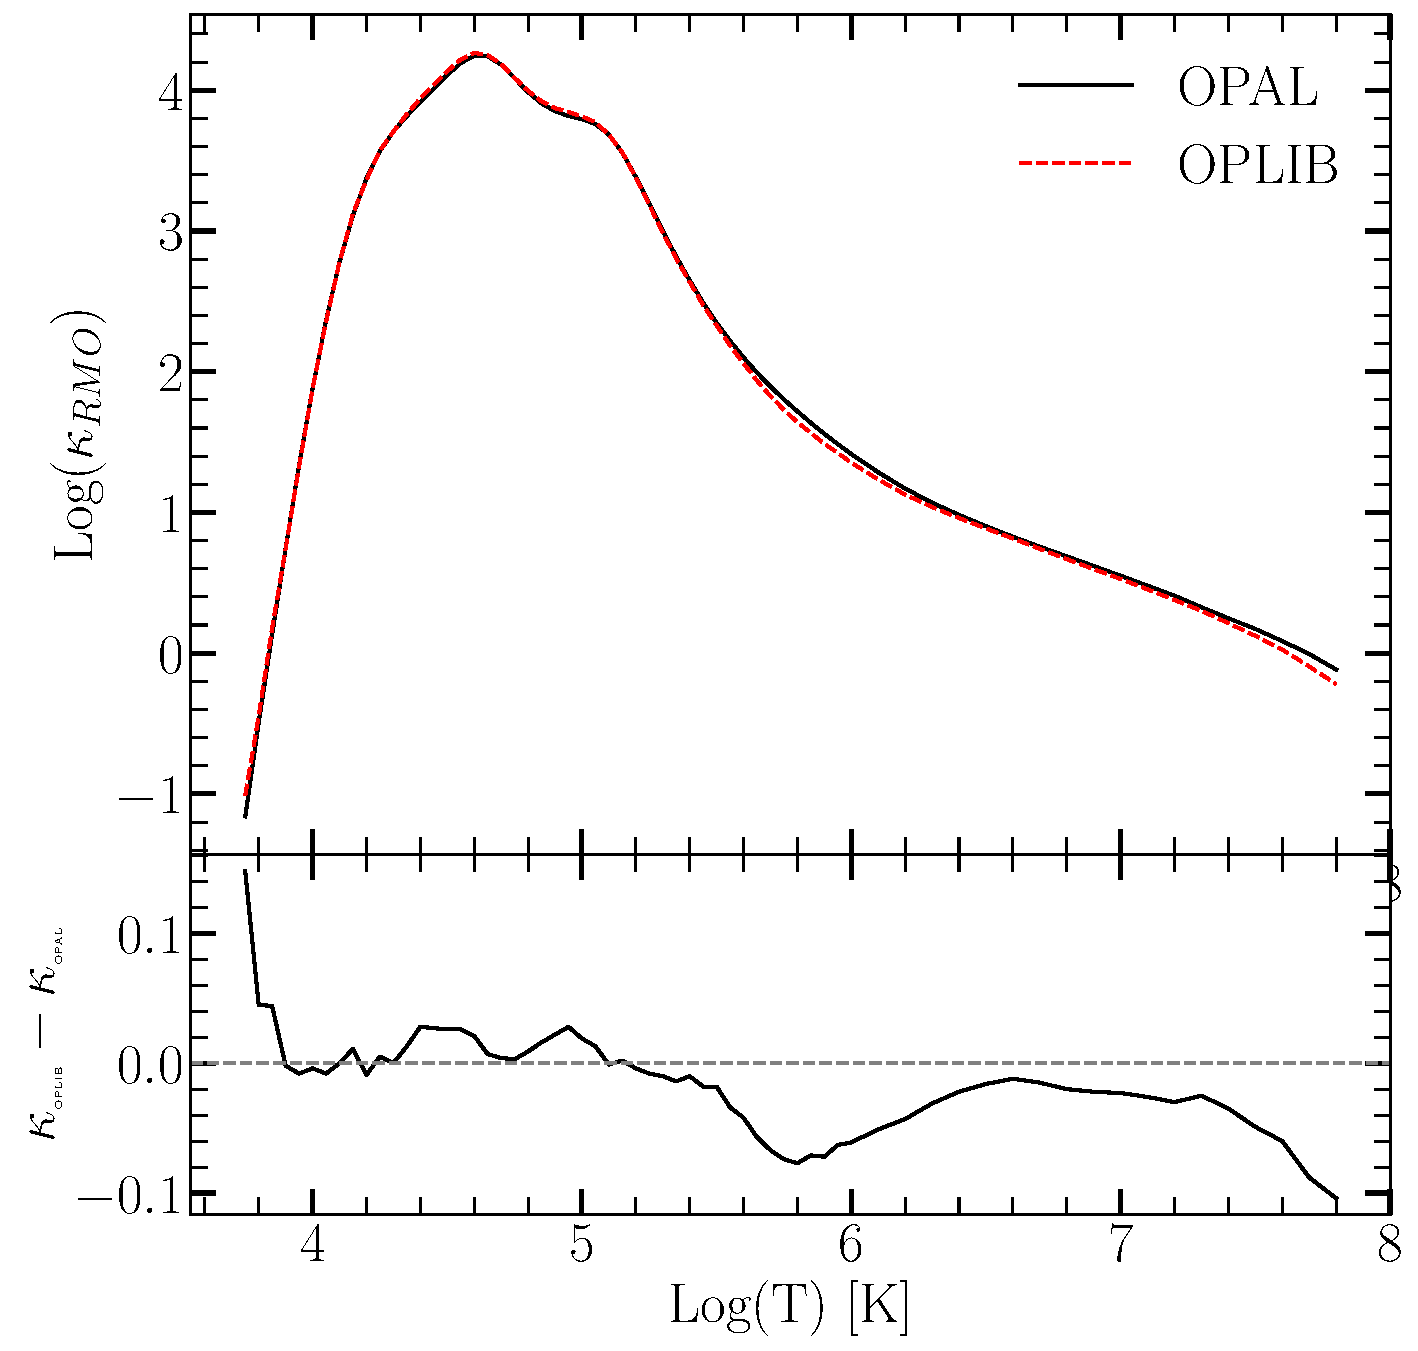
\includegraphics[width=0.45\textwidth]{figures/jaoOpacity/OpacityComparision.pdf}
	\caption{Rosseland mean opacity with the GS98 solar composition for both
	OPAL opacities and OPLIB opacities (top). Residuals between OPLIB opacities
	and OPAL opacities (bottom). These opacities are plotted at $\log _{10}(R)
	= -0.5$, $X=0.7$, and $Z=0.02$. $\log _{10}(R)=-0.5$ approximates
	much of the interior a 0.35 M$_{\odot}$ model. Note how the OPLIB
	opacities are systematically lower than the OPAL opacities for temperatures
	above $10^{5.2}$ K.}
	\label{fig:opacComp}
\end{figure}

\subsection{Table Querying and Conversion}
The high-temperature opacity tables used by DSEP and most other stellar
evolution programs give Rosseland-mean opacity, $\kappa_{R}$, along three
dimensions: temperature, a density proxy $R$ (Equation \ref{eqn:R}; $T_{6} =
T\times10^{-6}$, $\rho$ is the mass density), and composition. 

\begin{align} \label{eqn:R}
	R = \frac{\rho}{T_{6}^{3}}
\end{align}

OPLIB tables may be queried from a web
interface\footnote{https://aphysics2.lanl.gov/apps/}; however, OPLIB opacities
are parametrized using mass-density and temperature instead of $R$ and
temperature. It is most efficient for us to convert these tables to the OPAL
format instead of modifying DSEP to use the OPLIB format directly. In order to
generate many tables easily and quickly we develop a web scraper
\citep[\texttt{pyTOPSScrape},][]{Boudreaux22} which can automatically retrieve
all the tables needed to build an opacity table in the OPAL format.
\texttt{pyTOPSScrape}\footnote{https://github.com/tboudreaux/pytopsscrape} has
been released under the permissive \texttt{MIT} license with the consent of the
Los Alamos T-1 group. For a detailed discussion of how the web scraper works
and how OPLIB tables are transformed into a format DSEP can use see Appendices
\ref{apx:pytopsscrape} \& \ref{apx:interp}.

\subsection{Solar Calibrated Stellar Models}\label{sec:SCSM}
% In order to further validate the OPLIB high-temperature opacities we first visually
% compare a set of opacity vs. temperature curves from OPLIB at a constant $R$
% and \citet{Grevesse1998} composition (GS98) to the same curve from OPAL. A
% characteristic opacity vs temperature curve is shown in Figure
% \ref{fig:OpacCompare}, $\log _{10}(R) = -1.5$ is chosen as for much of the
% radius of a main sequence star $\log _{10}(R)$ is around that value. The
% largest variation in $\kappa_{R}$ from OPAL to OPLIB at $\log _{10}(R)=-1.5$ is
% on the order of a few percent. This is inline with expectations of OPLIB and OPAL
% being in relatively close agreement \citep{Colgan2016}.


In order to validate the OPLIB opacities, we generate a solar calibrated
stellar model (SCSM) using these new tables. We first manually calibrate the
surface Z/X abundance to within one part in 100 of the solar value \citep[][Z/X=0.23]{Grevesse1998}.
Subsequently, we allow both the convective mixing length parameter,
$\alpha_{ML}$, and the initial Hydrogen mass fraction, $X$, to vary
simultaneously, minimizing the difference, to within one part in $10^{5}$,
between resultant models' final radius and luminosity to those of the sun.
Finally, we confirm that the model's surface Z/X abundance is still within one
part in 100 of the solar value.

\begin{figure}
	\centering
	\includegraphics[width=0.45\textwidth]{figures/jaoOpacity/HRDiagramOPALvsOPLIB_SCCM.pdf}
	\caption{HR Diagram for the two SCSMs, OPAL and OPLIB. OPLIB is shown as a red
	dashed line.}
	\label{fig:OPLIBOPALHR}
\end{figure}

Solar calibrated stellar models evolved using GS98 OPAL and OPLIB opacity
tables (Figure \ref{fig:OPLIBOPALHR}) differ $\sim 0.5\%$ in the SCSM hydrogen
mass fractions and $\sim 1.5\%$ in the SCSM convective mixing length parameters
(Table \ref{tab:SCSMResults}). While the two evolutionary tracks are very
similar, note that the OPLIB SCSM's luminosity is systematically lower past the
solar age. While at the solar age the OPLIB SCSM luminosity is effectively the
same as the OPAL SCSM. This luminosity difference between OPAL and OPLIB based
models is not inconsistent with expectations given the more shallow radiative
temperature gradient resulting from the lower OPLIB opacities

\begin{table}
	\centering
	\begin{tabular}{l c c}
		\hline
		Model & $X$ & $\alpha_{ML}$ \\
		\hline
		\hline
		OPAL & 0.7066 & 1.9333 \\
		OPLIB & 0.7107 & 1.9629
	\end{tabular}
	\caption{Optimized parameters for SCSMs evolved using OPAL and OPLIB high
	temperature opacity tables.}
	\label{tab:SCSMResults}
\end{table}



% \section{Solar Calibrated Stellar Models}\label{sec:SCSM}
% In order to further validate the OPLIB high-temperature opacities we first visually
% compare a set of opacity vs. temperature curves from OPLIB at a constant $R$
% and \citet{Grevesse1998} composition (GS98) to the same curve from OPAL. A
% characteristic opacity vs temperature curve is shown in Figure
% \ref{fig:OpacCompare}, $\log _{10}(R) = -1.5$ is chosen as for much of the
% radius of a main sequence star $\log _{10}(R)$ is around that value. The
% largest variation in $\kappa_{R}$ from OPAL to OPLIB at $\log _{10}(R)=-1.5$ is
% on the order of a few percent. This is inline with expectations of OPLIB and OPAL
% being in relatively close agreement \citep{Colgan2016}.


In order to validate the OPLIB opacities, we generate a solar calibrated
stellar model (SCSM) using these new tables. We allow both the convective
mixing length parameter, $\alpha_{ML}$, and the initial Hydrogen mass fraction,
$X$, to vary simultaneously, minimizing the difference between resultant
models' final radius and luminosity to those of the sun.

Optimization of $\alpha_{ML}$ and $X$ is conducted using gradient descent. For
each optimization step three models are evolved: a reference model, a model
with a small perturbation to the hydrogen mass fraction but the same mixing
length as the reference model, and a model with a small perturbation to the
mixing length but the same hydrogen mass fraction as the reference.
Perturbations are sampled from a normal distribution (using
\texttt{numpy.random}). This distribution is sampled and that sample is then
added to the reference value for either $X$ or $\alpha_{ML}$. The luminosity
and radius of the three evolved models are compared to solar values and the
gradient of the resultant $L-L_{\odot}$, $R-R_{\odot}$ surface is followed down
to new estimates for the reference values of $X$ and $\alpha_{ML}$. This
process is is repeated until the difference between successive $X$ and
$\alpha_{ML}$ drops below one part in $10^{5}$.

\begin{figure}
	\centering
	\includegraphics[width=0.45\textwidth]{figures/jaoOpacity/src/figures/NotebookFigs/HRDiagramOPALvsOPLIB_SCCM.pdf}
	\caption{HR Diagram for the two SCSMs, OPAL and OPLIB. OPLIB is shown as a grey
	dashed line.}
	\label{fig:OPLIBOPALHR}
\end{figure}

Solar calibrated stellar models evolved using GS98 OPAL and OPLIB opacity
tables (Figure \ref{fig:OPLIBOPALHR}) differ $\sim 0.5\%$ in the SCSM hydrogen
mass fractions and $\sim 1.5\%$ in the SCSM convective mixing length parameters
(Table \ref{tab:SCSMResults}). While the two evolutionary tracks are very
similar, note that the OPLIB SCSM's luminosity is systematically lower at the
same age until the star leaves the main sequence, at which point it is
effectively the same as the OPAL SCSM. This luminosity difference between OPAL
and OPLIB based models is consistent with expectations given the shallow
radiative temperature gradient resulting from the lower OPLIB opacities

\begin{table}
	\centering
	\begin{tabular}{l c c}
		\hline
		Model & $X$ & $\alpha_{ML}$ \\
		\hline
		\hline
		OPAL & 0.7066 & 1.9333 \\
		OPLIB & 0.7107 & 1.9629
	\end{tabular}
	\caption{Optimized parameters for SCSMs evolved using OPAL and OPLIB high
	temperature opacity tables.}
	\label{tab:SCSMResults}
\end{table}


\section{Modeling}\label{sec:modeling}
In order to model the Jao Gap we evolve two extremely finely sampled mass grids
of models. One of these grids uses the OPAL high-temperature opacity tables
while the other uses the OPLIB tables (Figure \ref{fig:PunchIn}). Each grid
evolves a model every 0.00025 $M_{\odot}$ from 0.2 to 0.4 $M_{\odot}$ and every
0.005 $M_{\odot}$ from 0.4 to 0.8 $M_{\odot}$. All models in both grids use a
GS98 solar composition, the (1, 101, 0) \texttt{FreeEOS} (version
{\color{red}2.7}) configuration, and 1000 year old pre-main sequence polytropic
models, with polytropic index 1.5, as their initial conditions. We
include gravitational settling in our models where elements are grouped
together. Finally, we set a maximum allowed timestep of 50 million years to
assure that we fully resolve the build of of core $^{3}$He in gap stars.

Despite the alternative view of convection provided by
\citet{MacDonald2018} discussed in Section \ref{sec:JaoGap}, given that the
mixing timescales in these low mass stars are so short \citep[between $10^{7}$s
and $10^{8}$s per][Figure 2 \& Equation 39, which present the
averaged velocity over the convection zone]{Jermyn2022} instantaneous mixing is a valid
approximation. Moreover, one principal motivation for a diffusive model of
convective mixing has been to account for a deuterium concentration gradient
which \citet{Chabrier1997} identify will develop when the deuterium lifetime
against proton capture is significantly shorter than the mixing timescale.
However, the treatment of energy generation used by DSEP \citep{Bahcall2001}
avoides this issue by computing both the equilibrium deuterium abundance and
luminosity of each shell individually, implicitly accounting for the overall
luminosity discrepancy identified by \citeauthor{Chabrier1997}.

Because in this work we are just interested in the location shift of the Gap as
the opacity source varies, we do not model variations in composition.
\citet{Mansfield2021,Jao2020,Feiden2021} all look at the effect composition has
on Jao Gap location. They find that as population metallicity increases so too
does the mass range and consequently the magnitude of the Gap. From an extremely
low metallicity population (Z=0.001) to a population with a more solar like
metallicity this shift in mass range can be up to 0.05 M$_{\odot}$
\citep{Mansfield2021}.

\begin{figure}
	\centering
	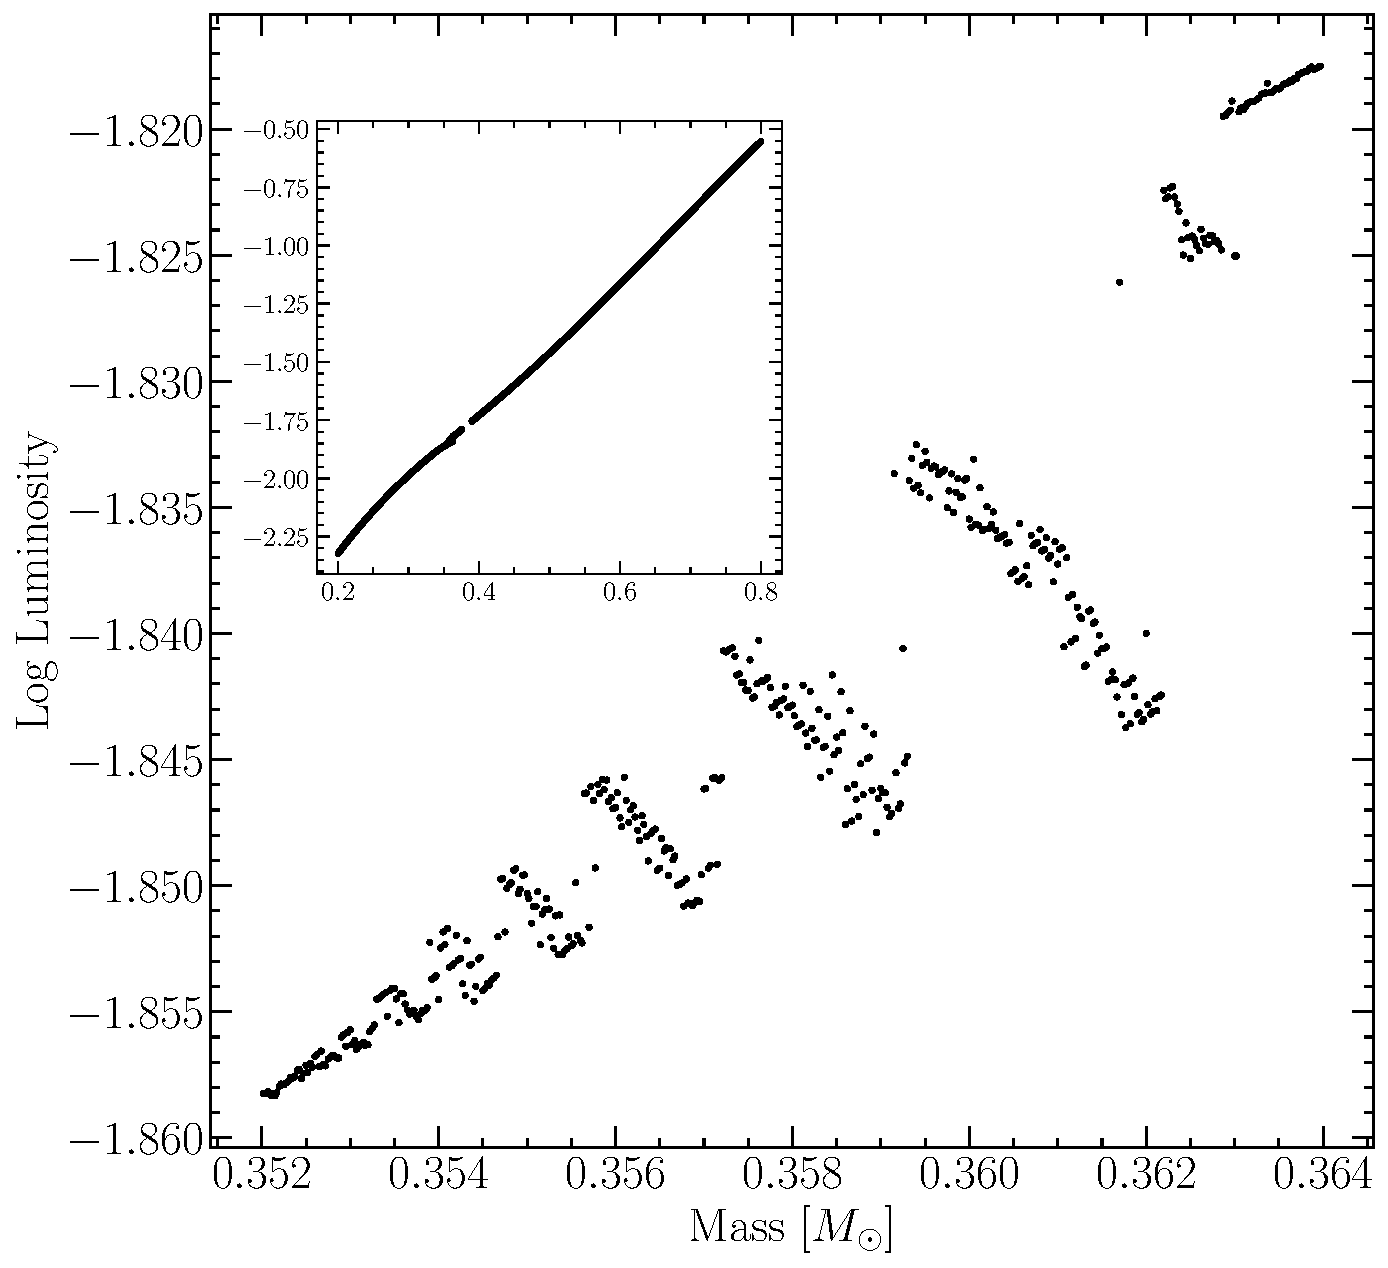
\includegraphics[width=0.85\textwidth]{figures/jaoOpacity/OPALPunchIn.pdf}
	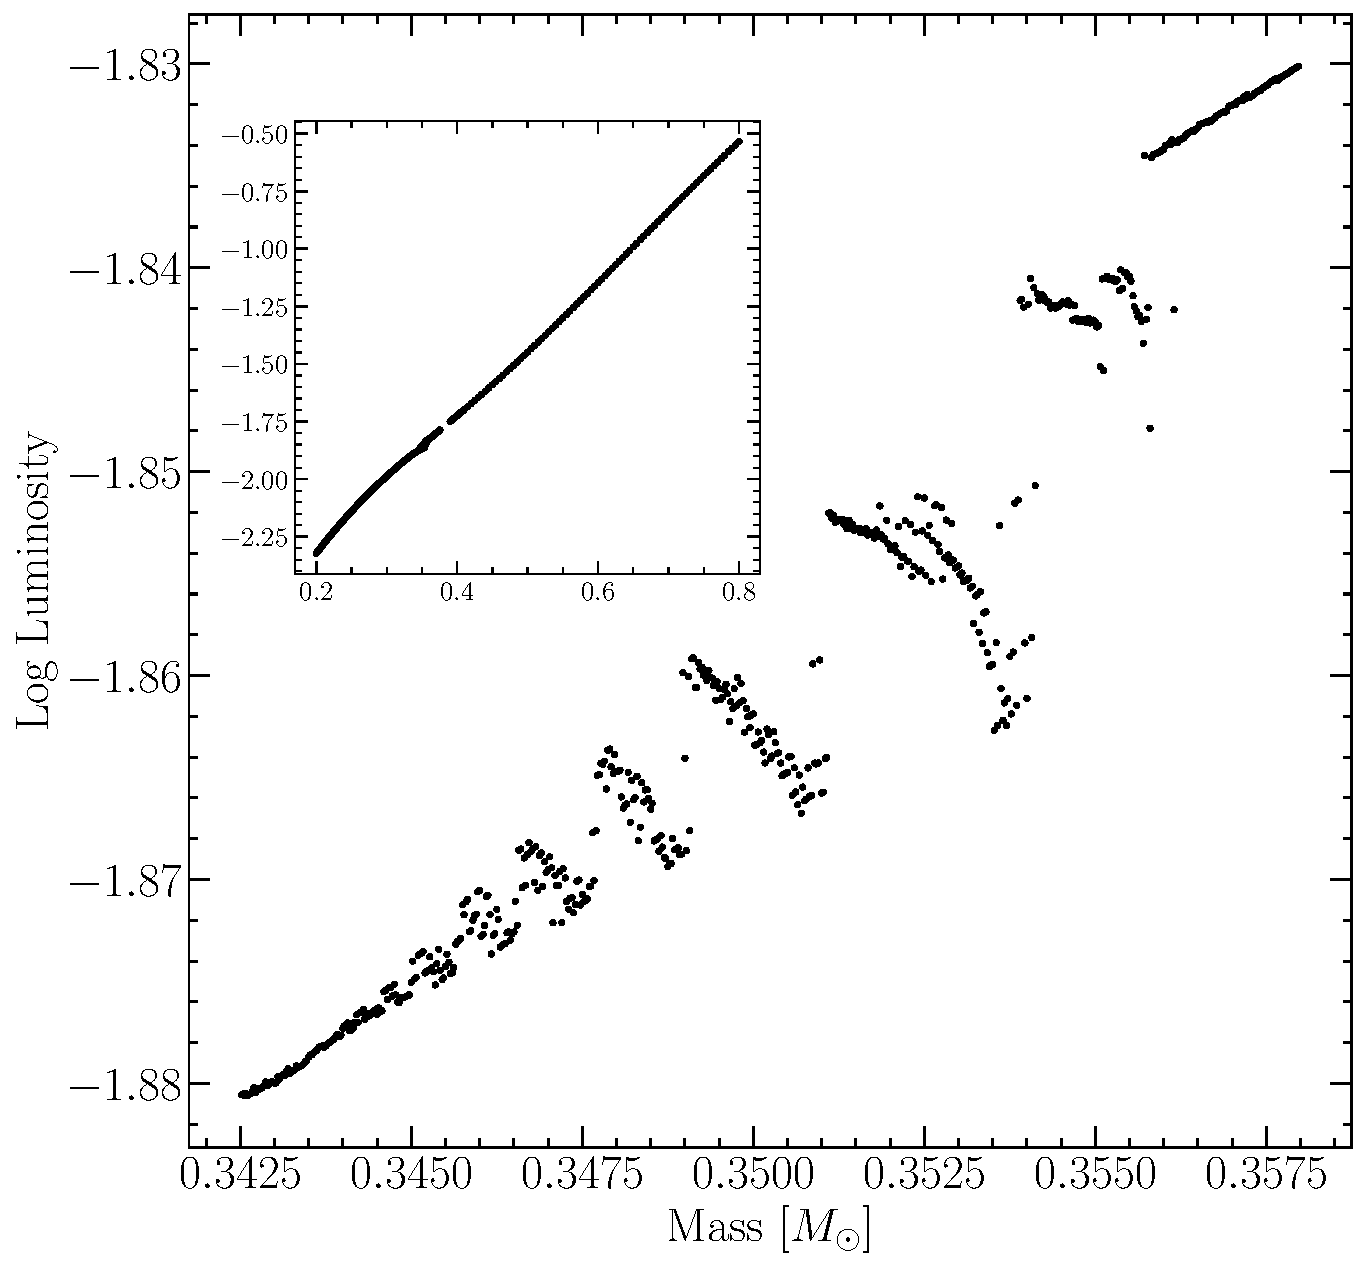
\includegraphics[width=0.85\textwidth]{figures/jaoOpacity/OPLIBPunchIn.pdf}
	\caption{Mass-luminosity relation at 7 Gyrs for models evolved using OPAL opacity
	tables (top) and those evolved using OPLIB opacity tables (bottom). Note
	the lower mass range of the OPLIB Gap.}
	\label{fig:PunchIn}
		
\end{figure}

\subsection{Population Synthesis}
In order to compare the Gap to observations we use in house population
synthesis code. We empirically calibrate the relation between G, BP, and RP
magnitudes and their uncertainties along with the parallax/G magnitude
uncertainty relation using the Gaia Catalouge of Nearby Stas
\citep[GCNS,][]{GaiaCollaboration2021} and Equations \ref{eqn:plxCalib} \&
\ref{eqn:MagCalib}. $M_{g}$ is the Gaia G magnitude while $M_{i}$ is the
magnitude in the i$^\text{th}$ band, G, BP, or RP. The coefficients $a$, $b$,
and $c$ determined using a non-linear least squares fitting routine. Equation
\ref{eqn:plxCalib} then models the relation between G magnitude and parallax
uncertainty while Equation \ref{eqn:MagCalib} models the relation between each
magnitude and its uncertainty.

\begin{align}\label{eqn:plxCalib}
	\sigma_{plx}(M_{g}) = ae^{bM_{g}}+c
\end{align}
\begin{align}\label{eqn:MagCalib}
	\sigma_{i}(M_{i}) = ae^{M_{i}-b}+c
\end{align}

\noindent The full series of steps in our population synthesis code
are:

\begin{figure}
	\centering
	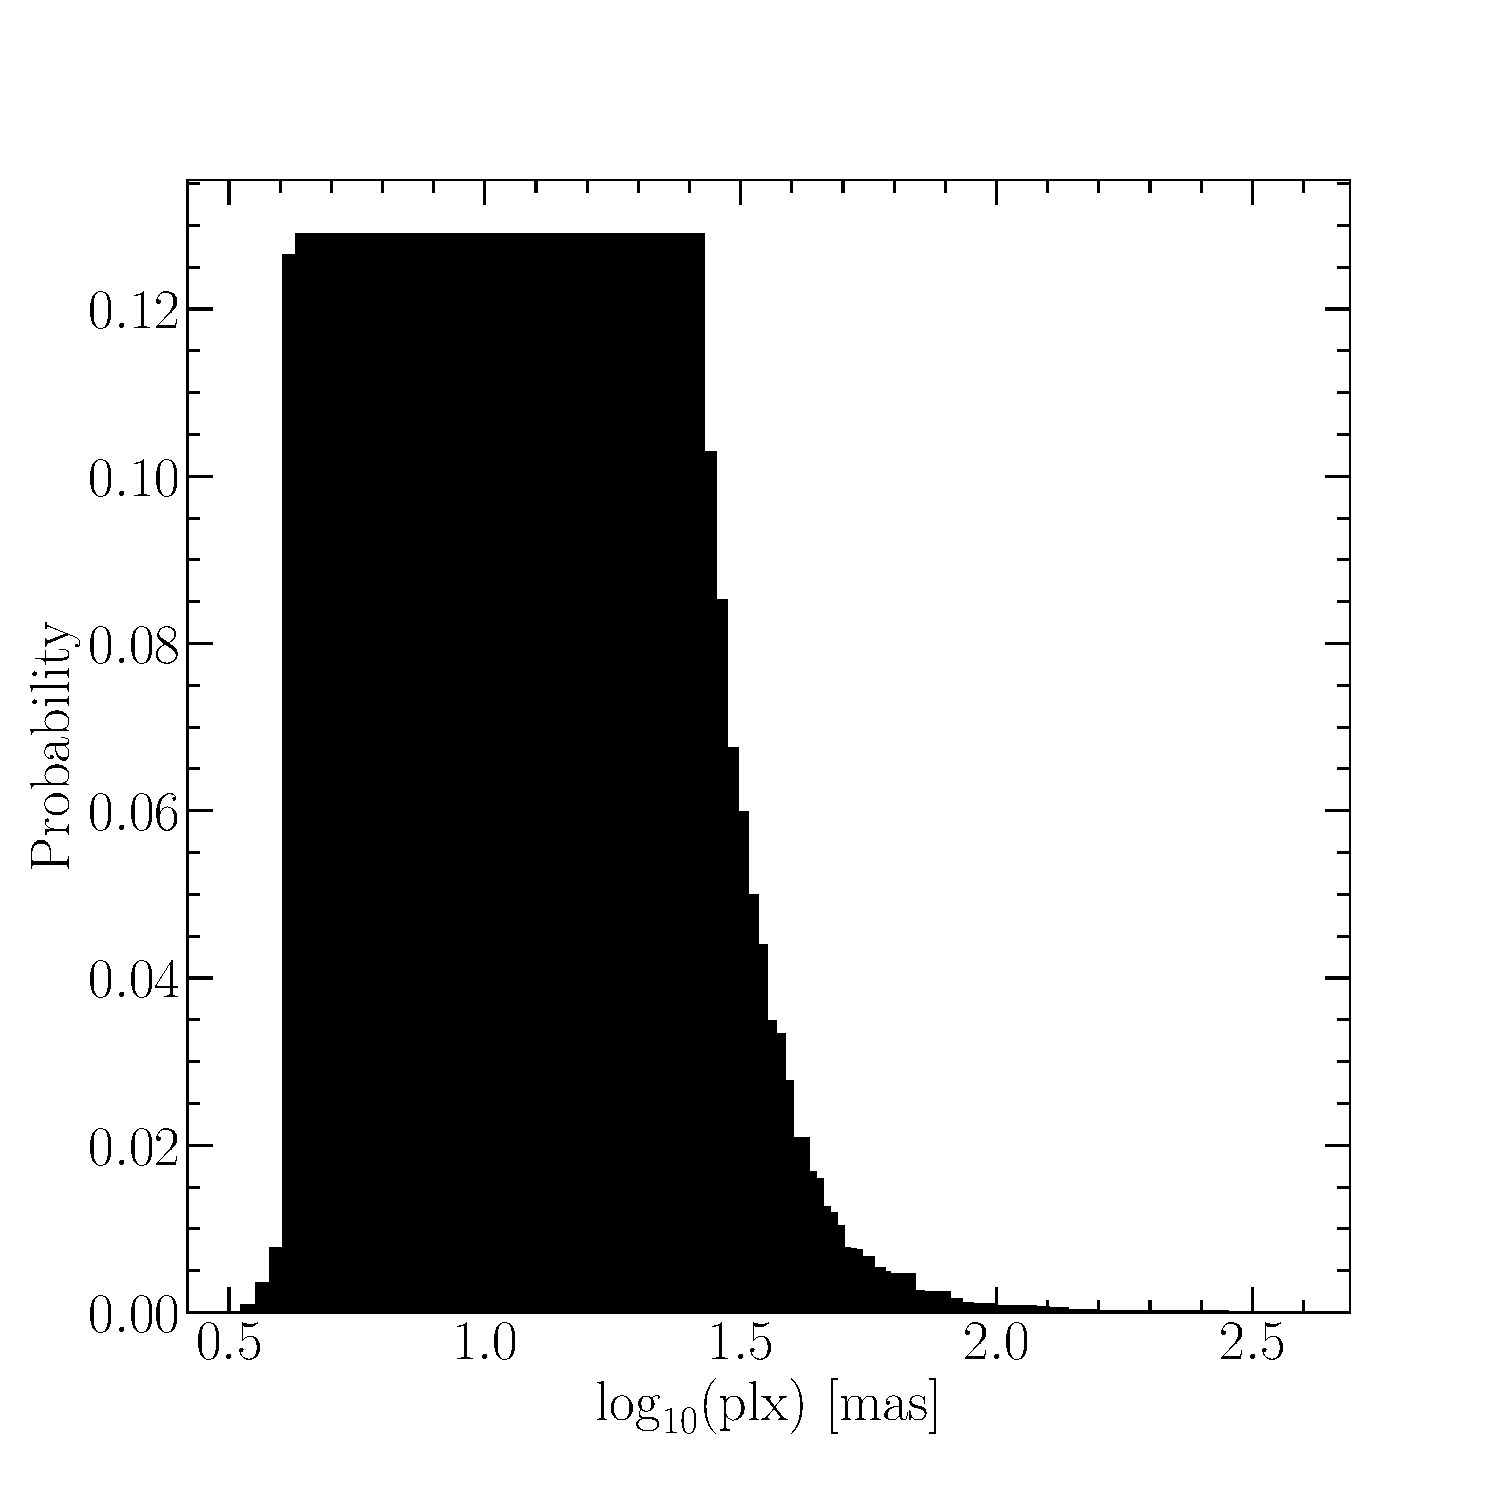
\includegraphics[width=0.85\textwidth]{figures/jaoOpacity/pdist.pdf}
	\caption{Probability distribution sampled when assigning true parallaxes to
	synthetic stars. This distribution is built from the GCNS and includes all
	stars with BP-RP colors between 2.3 and 2.9, the same color range
	of the Jao Gap.}
	\label{fig:pdist}
\end{figure}

\begin{enumerate}
	\item Sample from a \citet{Sollima2019} ($0.25 M_{\odot} < M < 1 M_{\odot}$,
		$\alpha=-1.34\pm0.07$) IMF to determine synthetic star mass.
	\item Find the closest model above and below the synthetic star, lineally
		interpolate these models' $T_{eff}$, $\log(g)$, and $\log(L)$ to those
		at the synthetic star mass.
	\item Convert synthetic star $g$, $T_{eff}$, and $Log(L)$ to Gaia G, BP,
		and RP magnitudes using the Gaia (E)DR3 bolometric corrections
		\citep{Creevey2022} along with code obtained thorough personal
		communication with Aaron Dotter \citep{Choi2016}.
	\item Sample from the GCNS parallax distribution (Figure \ref{fig:pdist}),
		limited to stars within the BP-RP color range of 2.3 -- 2.9, to assign
		synthetic star a ``true'' parallax.
	\item Use the true parallax to find an apparent magnitude for each filter.
	\item Evaluate the empirical calibration given in Equation
		\ref{eqn:plxCalib} to find an associated parallax uncertainty. Then
		sample from a normal distribution with a standard deviation equal to
		that uncertainty to adjust the true parallax resulting in an
		``observed'' parallax.
	\item Use the ``observed'' parallax and the apparent magnitude to find an
		``observed'' magnitude.
	\item Fit the empirical calibration given in Equation \ref{eqn:MagCalib} to
		the GCNS and evaluate it to give a magnitude uncertainty scale in each
		band.
	\item Adjust each magnitude by an amount sampled from a normal
		distribution with a standard deviation of the magnitude uncertainty
		scale found in the previous step.
\end{enumerate}

This method then incorporates both photometric and astrometric uncertainties
into our population synthesis. An example 7 Gyr old synthetic populations
using OPAL and OPLIB opacities are presented in Figure
\ref{fig:PopSynthCompareBasic}.

\begin{figure*}
	\centering
	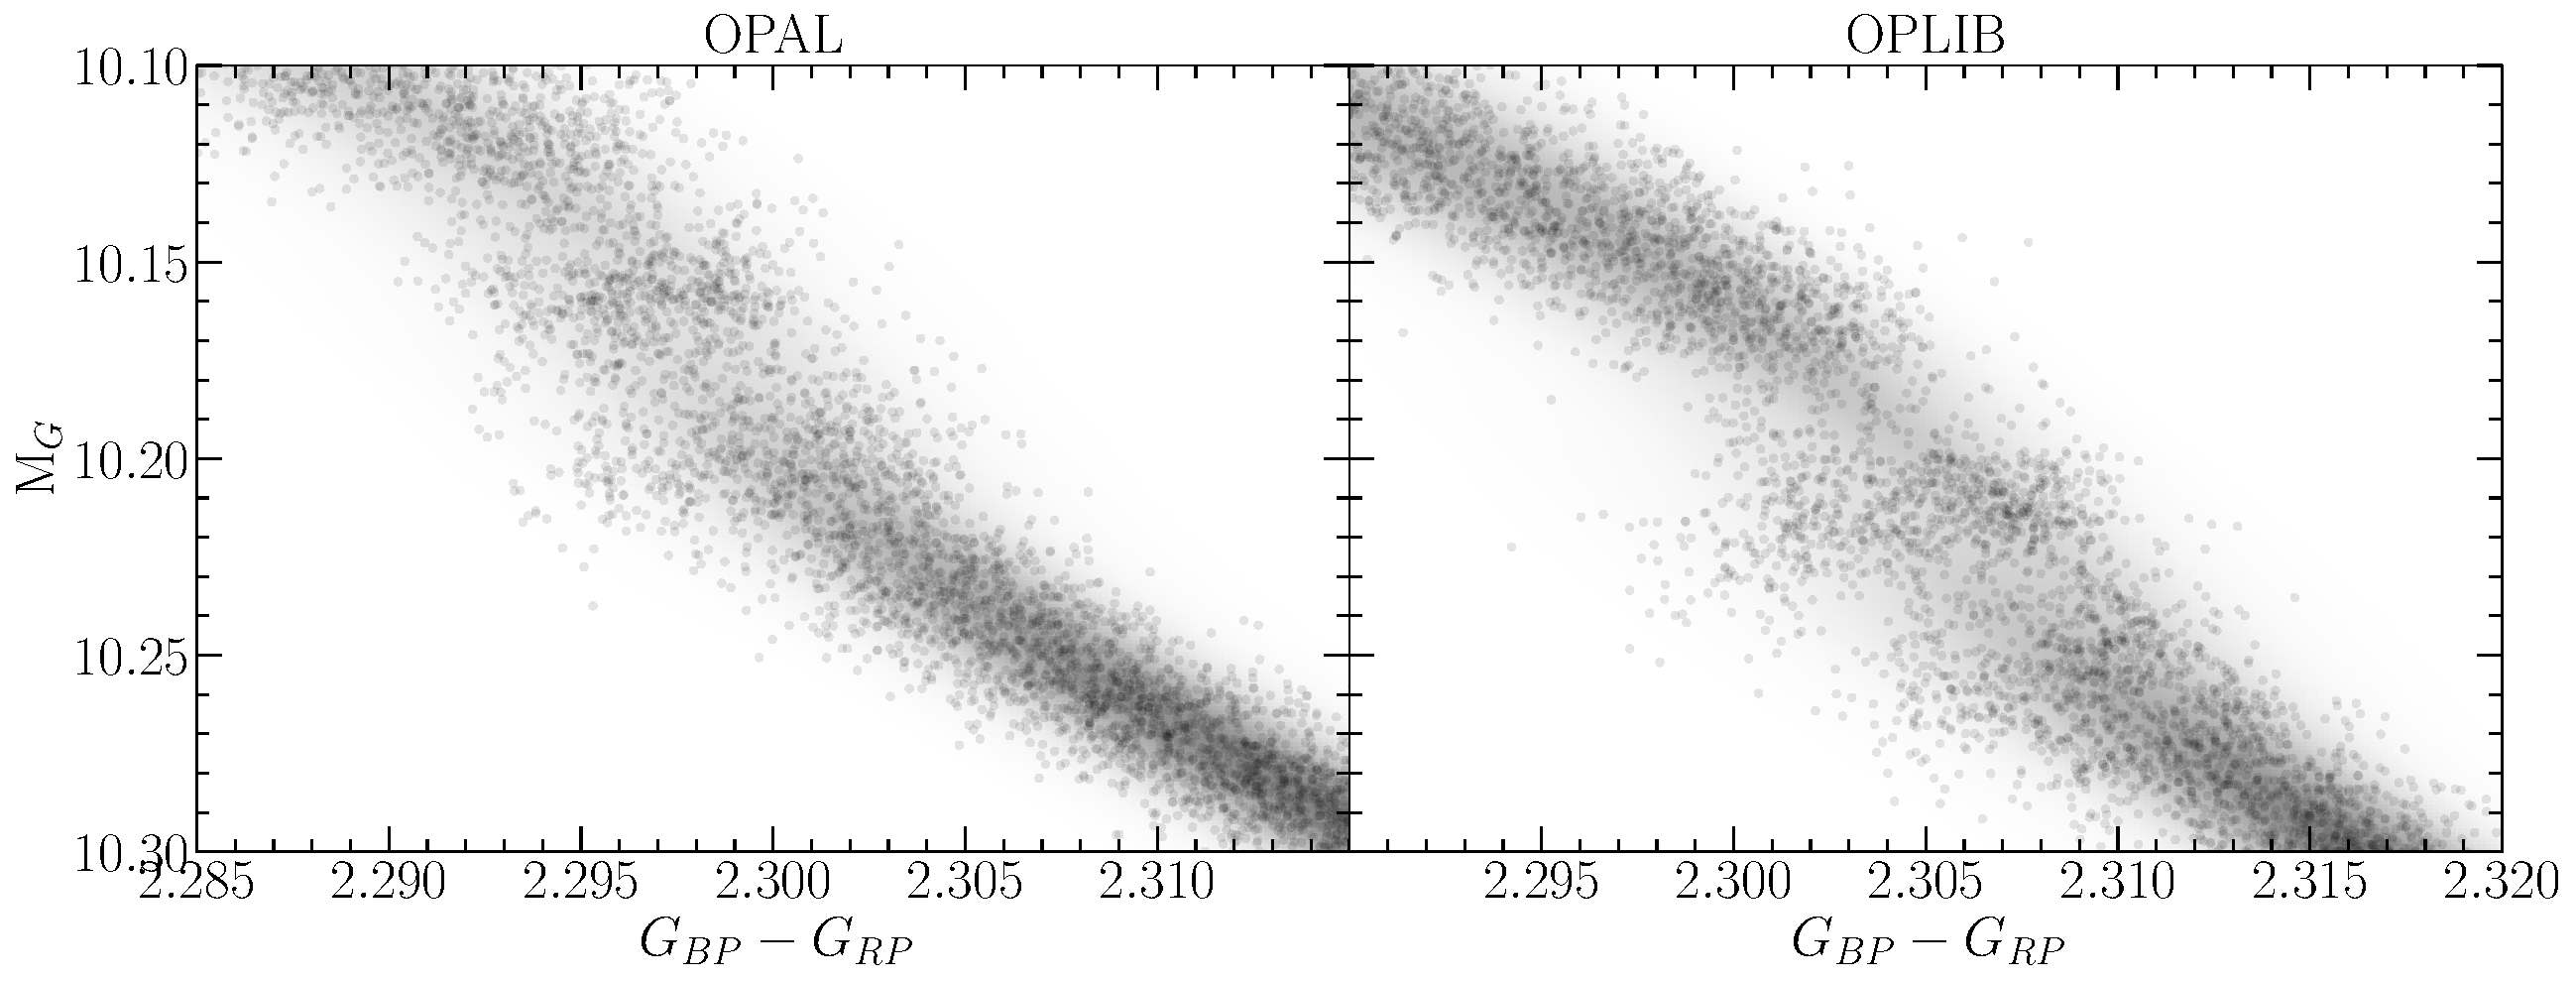
\includegraphics[width=0.85\textwidth]{figures/jaoOpacity/OPALOPLIB_popsynth_compare.pdf}
	\caption{Population synthesis results for models evolved with OPAL (left)
	and models evolved with OPLIB (right). A Gaussian kernel-density estimate
	has been overlaid to better highlight the density variations.}
	\label{fig:PopSynthCompareBasic}
\end{figure*}

\subsection{Mixing Length Dependence}
In order to test the sensitivity of Gap properties to mixing length we
evolve three separate sets OPLIB of models. The first uses a GS98
solar calibrated mixing length, the second uses a mixing length of
1.5, and the third uses a mixing length of 1.0.

We find a clear inverse correlation between mixing length parameter used and
the magnitude of the Jao Gap Figures \ref{fig:MixingLengthCMD} \&
\ref{fig:MixingLengthScaling} ($\mu_{G} \propto -1.5\alpha_{ML}$, where
$\mu_{G}$ is the mean magnitude of the Gap). This is somewhat surprising given
the long established view that the mixing length parameter is of little
relevance in fully convective stars \citep{Baraffe1997}. We find an approximate
0.3 magnitude shift in both the color and magnitude comparing a solar
calibrated mixing length to a mixing length of 1.5, despite only a 16K
difference in effective temperature at 7Gyr between two 0.3 solar mass models.
The slight temperature differences between these models are
attributable to the steeper adiabatic temperature gradients just below the
atmosphere in the solar calibrated mixing length model compared to the
$\alpha_{ML} = 1.5$ model ($\nabla_{ad,solar} - \nabla_{ad,1.5} \approx 0.05$).
Despite this relatively small temperature variance, the large magnitude
difference is expected due to the extreme sensitivity of the bolometric
corrections on effective temperature at these low temperatures. The
mixing length then provides a free parameter which may be used to shift the gap
location in order to better match observations without having a major impact on
the effective temperature of models. Moreover, recent work indicates that using
a solar calibrated mixing length is not appropriate for all stars
\citep[e.g.][]{Trampedach2014, Joyce2018}.

\begin{figure}
	\centering
	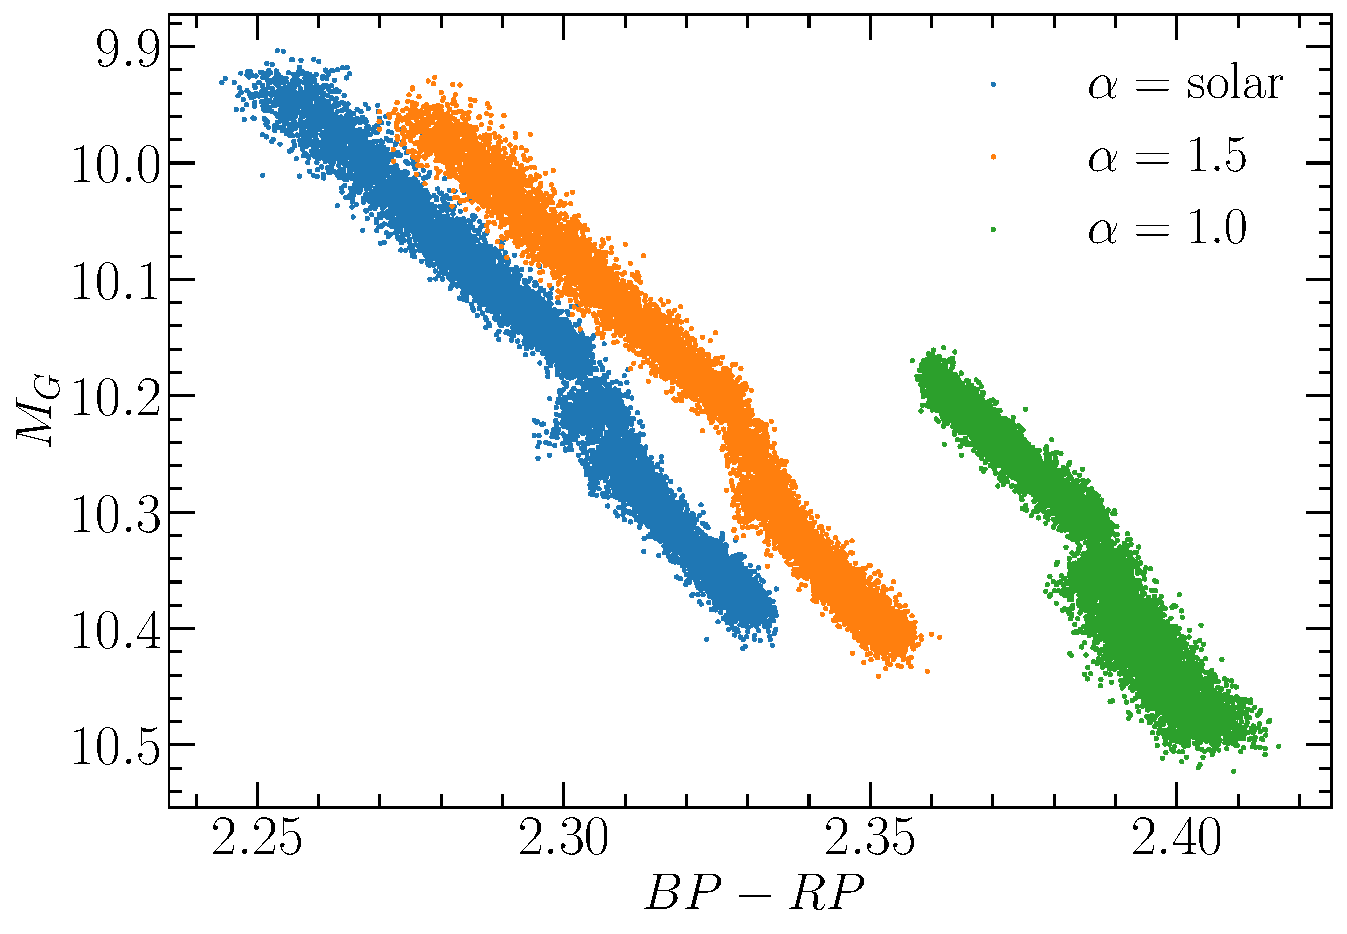
\includegraphics[width=0.85\textwidth]{figures/jaoOpacity/./alphaMLComparisionCMD.pdf}
	\caption{CMD showing OPLIB populations (from left to right) A, B, and C.}
	\label{fig:MixingLengthCMD}
\end{figure}

\begin{figure}
	\centering
	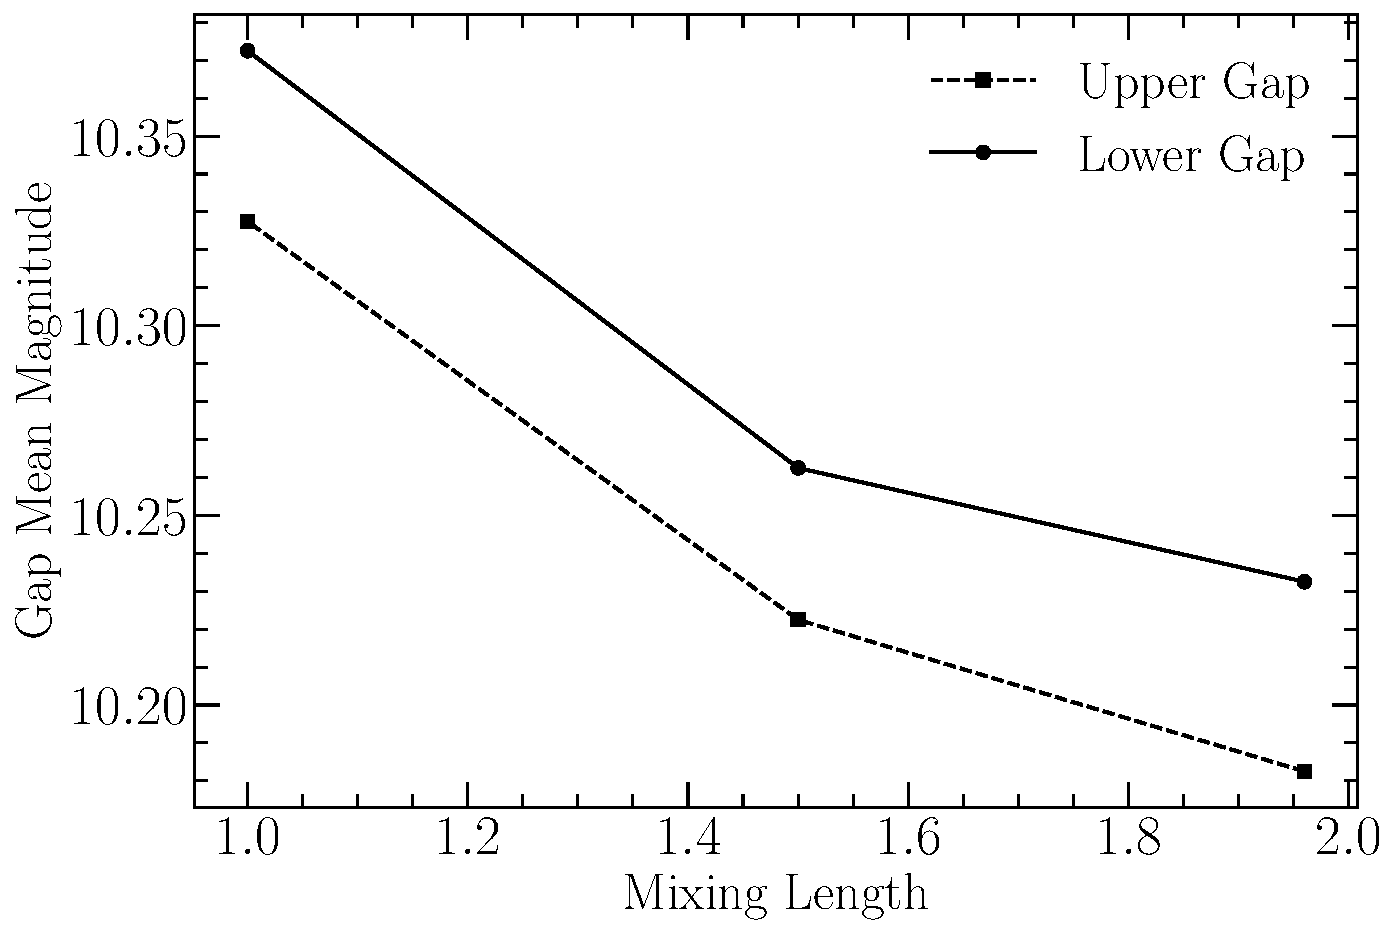
\includegraphics[width=0.85\textwidth]{figures/jaoOpacity/./MixingLengthScaling.pdf}
	\caption{Location of the two identified paucities of stars in OPLIB synthetic
	populations as a function of the mixing length used.}
	\label{fig:MixingLengthScaling}
\end{figure}

Given the variability of gap location with mixing length, it is possible that a
better fit to the gap location may be achieved through adjustment of the
convective mixing length parameter. However, calibrations of the mixing length
for stars other than the sun have focused on stars with effective temperature
at or above that of the sun and there are no current calibrations of the mixing
length parameter for M dwarfs. Moreover, there are additional uncertainties
when comparing the predicted gap location to the measured gap location, such as
those in the conversion from effective temperature, surface gravity, and
luminosity to color, which must be considered if the mixing length is to be
used as a gap location free parameter. Given the dangers of freely adjustable
parameters and the lack of an a priori expectation for what the convective
mixing parameter should be for the population of M Dwarfs in the Gaia DR2 and
EDR3 CMD any attempt to use the Jao Gap magnitude to calibrate a mixing length
value must be done with caution, and take into account the other uncertainties
in the stellar models which could affect the Jao Gap magnitude.



\section{Rotation--Activity Relation}\label{sec:results}
We show our rotation-activity relation in Figures
\ref{fig:RpHKvsRossbySelf} \& \ref{fig:RpHKvsRossbyDef}. Note that
errors are shown in both figures; however, they render smaller than the data
point size. Ca II H\&K is also known to be time variable
\citep[e.g.][]{Baroch2020,Perdelwitz2021}, which is not captured in our
single-epoch data. There is one target cut off by the domain of this graph,
2MASS J10252645+0512391. This target has a measured vsini of $59.5\pm2.1$ km
s$^{-1}$ \citep{Kesseli2018} and is therefore quite rotationally broadened, which
is known to affect $R'_{HK}$ measurements \citep[figure 8]{Schroder2009}. The
data used to generate this figure is given in Table \ref{tab:finalData}. Table
\ref{tab:finalData} includes uncertainties, the R'$_{HK}$ measurements for
stars which did not have photometrically derived rotational periods in MEarth,
and data for 2MASS J10252645+0512391

We find a rotation activity relationship qualitatively similar to that
presented in \citet{Def17}. Our rotation activity relationship exhibits both
the expected saturated and unsaturated regimes --- the flat region at $Ro <
Ro_{s}$ and the sloped region at $Ro \geq Ro_{s}$ respectively. We fit the
rotation activity relation given in Equation \ref{eqn:fitEqn} to our data using
Markov Chain Monte Carlo (MCMC), implemented in \texttt{pymc}
\citep{Salvatier2016}. 

  \begin{equation}\label{eqn:fitEqn}
      \log(R'_{HK}) = \begin{cases}
          \log(R_{s}) & Ro < Ro_{s} \\
          k\log(Ro) + \log(R_{s}) - k\log(Ro_{s}) & Ro \geq Ro_{s}
      \end{cases}
  \end{equation}

\noindent $Ro_{s}$ is the Rossby number cutoff between the saturated and
unsaturated regime. $R_{s}$ is the maximum, saturated, value of $R'_{HK}$ and
$k$ is the index of the power law when $Ro \geq Ro_{s}$. Due to the
issues measuring $R'_{HK}$ for high vsini targets discussed above, we exclude
2MASS J10252645+0512391 from this fit. All logarithms are base ten unless
another base is explicitly given.
\begin{table}[ht]
  \small
    \centering
    \setlength{\tabcolsep}{4pt}
    \begin{tabular}{lcccccccc}
\hline
2MASS ID & Mass & $Ro$ & $\log(R'_{HK})$ & $\log(R'_{HK})_{err}$ & $V_{mag}$ & $V-K$ & prot & $r_{prot}$\\
 & $\mathrm{M_{\odot}}$ &  &  &  & $\mathrm{mag}$ & $\mathrm{mag}$ & $\mathrm{d}$ &   \\
\hline
\hline
06000351+0242236 & 0.24 & 0.020 & -4.5475 & 0.0021 & 11.31 & 5.268 & 1.809 & 2016ApJ...821...93N  \\
02125458+0000167 & 0.27 & 0.048 & -4.6345 & 0.0014 & 13.58 & 5.412 & 4.732 & 2016ApJ...821...93N  \\
01124752+0154395 & 0.28 & 0.026 & -4.4729 & 0.0017 & 14.009 & 5.240 & 2.346 & 2016ApJ...821...93N  \\
10252645+0512391 & 0.11 & 0.000 & -4.9707 & 0.0380 & 18.11 & 7.322 & 0.102 & 2016ApJ...821...93N  \\
05015746-0656459 & 0.17 & 0.873 & -5.0049 & 0.0028 & 12.2 & 5.464 & 88.500 & 2012AcA....62...67K  \\
06022261-2019447 & 0.23 & 1.307 & -5.6980 & 0.0192 & 13.26 & 4.886 & 95.000 & This Work  \\
06105288-4324178 & 0.30 & 0.705 & -5.2507 & 0.0139 & 12.28 & 4.968 & 53.736 & 2018AJ....156..217N  \\
09442373-7358382 & 0.24 & 0.542 & -5.6026 & 0.0147 & 15.17 & 5.795 & 66.447 & 2018AJ....156..217N  \\
14211512-0107199 & 0.24 & 1.160 & -5.5846 & 0.0125 & 13.12 & 5.027 & 91.426 & 2018AJ....156..217N  \\
14294291-6240465 & 0.12 & 0.394 & -5.0053 & 0.0014 & 11.13 & 6.746 & 83.500 & 1998AJ....116..429B  \\
16352464-2718533 & 0.23 & 1.423 & -5.5959 & 0.0108 & 14.18 & 5.182 & 122.656 & 2018AJ....156..217N  \\
16570570-0420559 & 0.24 & 0.014 & -4.3071 & 0.0014 & 12.25 & 5.130 & 1.212 & 2012AcA....62...67K  \\
02004725-1021209 & 0.34 & 0.188 & -4.7907 & 0.0026 & 14.118 & 5.026 & 14.793 & 2018AJ....156..217N  \\
18494929-2350101 & 0.18 & 0.034 & -4.5243 & 0.0015 & 10.5 & 5.130 & 2.869 & 2007AcA....57..149K  \\
20035892-0807472 & 0.33 & 0.946 & -5.6530 & 0.0077 & 13.54 & 5.254 & 84.991 & 2018AJ....156..217N  \\
21390081-2409280 & 0.21 & 1.152 & -6.1949 & 0.0190 & 13.45 & 5.091 & 94.254 & 2018AJ....156..217N  \\
23071524-2307533 & 0.30 & 0.720 & -5.2780 & 0.0077 & 13.587 & 4.849 & 51.204 & 2018AJ....156..217N  \\
00094508-4201396 & 0.30 & 0.009 & -4.3392 & 0.0018 & 13.62 & 5.397 & 0.859 & 2018AJ....156..217N  \\
00310412-7201061 & 0.31 & 0.906 & -5.3879 & 0.0074 & 13.69 & 5.245 & 80.969 & 2018AJ....156..217N  \\
01040695-6522272 & 0.17 & 0.006 & -4.4889 & 0.0024 & 13.98 & 5.448 & 0.624 & 2018AJ....156..217N  \\
02014384-1017295 & 0.19 & 0.034 & -4.5400 & 0.0022 & 14.473 & 5.284 & 3.152 & 2018AJ....156..217N  \\
03100305-2341308 & 0.40 & 0.028 & -4.2336 & 0.0017 & 13.502 & 4.935 & 2.083 & 2018AJ....156..217N  \\
03205178-6351524 & 0.33 & 1.029 & -5.6288 & 0.0096 & 13.433 & 5.238 & 91.622 & 2018AJ....156..217N  \\
07401183-4257406 & 0.15 & 0.002 & -4.3365 & 0.0022 & 13.81 & 6.042 & 0.307 & 2018AJ....156..217N  \\
08184619-4806172 & 0.37 & 0.021 & -4.2834 & 0.0025 & 14.37 & 5.019 & 1.653 & 2018AJ....156..217N  \\
08443891-4805218 & 0.20 & 1.348 & -5.6682 & 0.0067 & 13.932 & 5.370 & 129.513 & 2018AJ....156..217N  \\
09342791-2643267 & 0.19 & 0.007 & -4.3415 & 0.0025 & 13.992 & 5.373 & 0.694 & 2018AJ....156..217N  \\
09524176-1536137 & 0.26 & 1.342 & -5.6319 & 0.0110 & 13.43 & 4.923 & 99.662 & 2018AJ....156..217N  \\
11075025-3421003 & 0.25 & 0.068 & -4.2250 & 0.0032 & 15.04 & 5.633 & 7.611 & 2018AJ....156..217N  \\
11575352-2349007 & 0.39 & 0.031 & -4.2952 & 0.0026 & 14.77 & 5.415 & 3.067 & 2018AJ....156..217N  \\
12102834-1310234 & 0.36 & 0.435 & -4.6892 & 0.0029 & 13.83 & 5.418 & 42.985 & 2018AJ....156..217N  \\
12440075-1110302 & 0.18 & 0.020 & -4.4053 & 0.0033 & 14.22 & 5.546 & 2.099 & 2018AJ....156..217N  \\
13442092-2618350 & 0.35 & 2.032 & -5.9634 & 0.0253 & 13.253 & 4.968 & 154.885 & 2018AJ....156..217N  \\
14253413-1148515 & 0.51 & 0.301 & -4.7641 & 0.0030 & 13.512 & 5.121 & 25.012 & 2018AJ....156..217N  \\
14340491-1824106 & 0.38 & 0.271 & -4.6093 & 0.0038 & 14.346 & 5.638 & 30.396 & 2018AJ....156..217N  \\
15154371-0725208 & 0.38 & 0.050 & -4.6214 & 0.0023 & 12.93 & 5.224 & 4.379 & 2018AJ....156..217N  \\
15290145-0612461 & 0.46 & 0.095 & -4.2015 & 0.0017 & 14.011 & 5.230 & 8.434 & 2018AJ....156..217N  \\
16204186-2005139 & 0.45 & 0.031 & -4.3900 & 0.0035 & 13.68 & 5.261 & 2.814 & 2018AJ....156..217N  \\
16475517-6509116 & 0.17 & 0.889 & -4.8744 & 0.0045 & 13.98 & 5.101 & 73.142 & 2018AJ....156..217N  \\
20091824-0113377 & 0.15 & 0.010 & -4.3772 & 0.0023 & 14.47 & 5.958 & 1.374 & 2018AJ....156..217N  \\
20273733-5452592 & 0.35 & 1.520 & -5.9982 & 0.0181 & 13.18 & 5.259 & 136.924 & 2018AJ....156..217N  \\
20444800-1453208 & 0.49 & 0.073 & -4.4912 & 0.0023 & 14.445 & 5.305 & 6.715 & 2018AJ....156..217N  \\
15404341-5101357 & 0.10 & 0.318 & -5.0062 & 0.0081 & 15.26 & 7.317 & 93.702 & 2018AJ....156..217N  \\
22480446-2422075 & 0.20 & 0.005 & -4.4123 & 0.0016 & 12.59 & 5.384 & 0.466 & 2013AJ....146..154M  \\
06393742-2101333 & 0.26 & 0.952 & -5.2524 & 0.0069 & 12.77 & 5.120 & 79.152 & 2018AJ....156..217N  \\
04130560+1514520 & 0.30 & 0.019 & -4.4775 & 0.0088 & 15.881 & 5.437 & 1.881 & 2016ApJ...818..46M  \\
02411510-0432177 & 0.20 & 0.004 & -4.4272 & 0.0016 & 13.79 & 5.544 & 0.400 & 2020ApJ...905..107M  \\
  11381671-7721484 & 0.12 & 0.958 & \textbf{-5.5015} & 0.0369 & 14.78 & 6.259 & 153.506 & This Work  \\
  12384914-3822527 & 0.15 & 2.527 & \textbf{-6.0690} & 0.0156 & 12.75 & 5.364 & 241.913 & This Work  \\
  13464102-5830117 & 0.48 & 1.340 & \textbf{-5.6977} & 0.0146 &  &  & 65.017 & This Work  \\
  15165576-0037116 & 0.31 & 0.157 & \textbf{-4.0704} & 0.0024 & 14.469 & 5.364 & 15.028 & This Work  \\
  19204795-4533283 & 0.18 & 1.706 & \textbf{-5.8392} & 0.0091 & 12.25 & 5.405 & 167.225 & This Work  \\
  21362532-4401005 & 0.20 & 1.886 & \textbf{-5.8978} & 0.0168 & 14.14 & 5.610 & 207.983 & This Work  \\
\hline
\end{tabular}


% \begin{tabular}{lcccccc}
% \hline
% 	2MASS ID &  Mass &    $Ro$ &  $\log(R'_{HK})$ & $\log(R'_{HK})_{err}$ & $V_{mag}$ &   $V-K$ \\
% \hline
% \hline
% 06000351+0242236 &  0.237 &  0.020 &     -4.548 &          0.002 &  11.310 &  5.268 \\
% 02125458+0000167 &  0.268 &  0.048 &     -4.635 &          0.001 &  13.580 &  5.412 \\
% 01124752+0154395 &  0.278 &  0.026 &     -4.473 &          0.001 &  14.009 &  5.240 \\
% 10252645+0512391 &  0.111 &  0.000 &     -4.971 &          0.007 &  18.110 &  7.322 \\
% 05015746-0656459 &  0.168 &  0.873 &     -5.005 &          0.003 &  12.200 &  5.464 \\
% 06022261-2019447 &  0.234 &  1.307 &     -5.698 &          0.012 &  13.260 &  4.886 \\
% 06105288-4324178 &  0.295 &  0.705 &     -5.251 &          0.008 &  12.280 &  4.968 \\
% 09442373-7358382 &  0.240 &  0.542 &     -5.603 &          0.006 &  15.170 &  5.795 \\
% 14211512-0107199 &  0.238 &  1.160 &     -5.585 &          0.008 &  13.120 &  5.027 \\
% 14294291-6240465 &  0.119 &  0.394 &     -5.005 &          0.001 &  11.130 &  6.746 \\
% 16352464-2718533 &  0.228 &  1.423 &     -5.596 &          0.006 &  14.180 &  5.182 \\
% 16570570-0420559 &  0.242 &  0.014 &     -4.307 &          0.001 &  12.250 &  5.130 \\
% 02004725-1021209 &  0.343 &  0.188 &     -4.791 &          0.002 &  14.118 &  5.026 \\
% 18494929-2350101 &  0.175 &  0.034 &     -4.524 &          0.001 &  10.500 &  5.130 \\
% 20035892-0807472 &  0.328 &  0.946 &     -5.653 &          0.007 &  13.540 &  5.254 \\
% 21390081-2409280 &  0.209 &  1.152 &     -6.195 &          0.015 &  13.450 &  5.091 \\
% 23071524-2307533 &  0.303 &  0.720 &     -5.278 &          0.006 &  13.587 &  4.849 \\
% 00094508-4201396 &  0.304 &  0.009 &     -4.339 &          0.001 &  13.620 &  5.397 \\
% 00310412-7201061 &  0.311 &  0.906 &     -5.388 &          0.006 &  13.690 &  5.245 \\
% 01040695-6522272 &  0.171 &  0.006 &     -4.489 &          0.002 &  13.980 &  5.448 \\
% 02014384-1017295 &  0.193 &  0.034 &     -4.540 &          0.002 &  14.473 &  5.284 \\
% 03100305-2341308 &  0.395 &  0.028 &     -4.234 &          0.001 &  13.502 &  4.935 \\
% 03205178-6351524 &  0.330 &  1.029 &     -5.629 &          0.007 &  13.433 &  5.238 \\
% 07401183-4257406 &  0.154 &  0.002 &     -4.337 &          0.001 &  13.810 &  6.042 \\
% 08184619-4806172 &  0.370 &  0.021 &     -4.283 &          0.001 &  14.370 &  5.019 \\
% 08443891-4805218 &  0.202 &  1.348 &     -5.668 &          0.004 &  13.932 &  5.370 \\
% 09342791-2643267 &  0.192 &  0.007 &     -4.341 &          0.001 &  13.992 &  5.373 \\
% 09524176-1536137 &  0.264 &  1.342 &     -5.632 &          0.007 &  13.430 &  4.923 \\
% 11075025-3421003 &  0.255 &  0.068 &     -4.225 &          0.001 &  15.040 &  5.633 \\
% 11575352-2349007 &  0.393 &  0.031 &     -4.295 &          0.001 &  14.770 &  5.415 \\
% 12102834-1310234 &  0.355 &  0.435 &     -4.689 &          0.002 &  13.830 &  5.418 \\
% 12440075-1110302 &  0.184 &  0.020 &     -4.405 &          0.002 &  14.220 &  5.546 \\
% 13442092-2618350 &  0.348 &  2.032 &     -5.963 &          0.014 &  13.253 &  4.968 \\
% 14253413-1148515 &  0.505 &  0.301 &     -4.764 &          0.002 &  13.512 &  5.121 \\
% 14340491-1824106 &  0.377 &  0.271 &     -4.609 &          0.002 &  14.346 &  5.638 \\
% 15154371-0725208 &  0.378 &  0.050 &     -4.621 &          0.002 &  12.930 &  5.224 \\
% 15290145-0612461 &  0.455 &  0.095 &     -4.201 &          0.001 &  14.011 &  5.230 \\
% 16204186-2005139 &  0.453 &  0.031 &     -4.390 &          0.002 &  13.680 &  5.261 \\
% 16475517-6509116 &  0.170 &  0.889 &     -4.874 &          0.003 &  13.980 &  5.101 \\
% 20091824-0113377 &  0.147 &  0.010 &     -4.377 &          0.001 &  14.470 &  5.958 \\
% 20273733-5452592 &  0.350 &  1.520 &     -5.998 &          0.012 &  13.180 &  5.259 \\
% 20444800-1453208 &  0.485 &  0.073 &     -4.491 &          0.002 &  14.445 &  5.305 \\
% 15404341-5101357 &  0.098 &  0.318 &     -5.006 &          0.003 &  15.260 &  7.317 \\
% 22480446-2422075 &  0.198 &  0.005 &     -4.412 &          0.001 &  12.590 &  5.384 \\
% 06393742-2101333 &  0.258 &  0.952 &     -5.252 &          0.004 &  12.770 &  5.120 \\
% 04130560+1514520 &  0.298 &  0.019 &     -4.477 &          0.004 &  15.881 &  5.437 \\
% 02411510-0432177 &  0.197 &  0.004 &     -4.427 &          0.001 &  13.790 &  5.544 \\
% \hline
% \end{tabular}

% \begin{tabular}{lccccc}
% \hline
% 2MASS ID &  Mass &    $Ro$ &  $\log(R'_{HK})$ &   $V_{mag}$ &   V-K \\
% \hline
% \hline
% J00094508-4201396 &  0.30 &  0.01 &      -4.33 &  13.62 &  5.40 \\
% J00310412-7201061 &  0.31 &  0.91 &      -5.36 &  13.69 &  5.24 \\
% J01040695-6522272 &  0.17 &  0.01 &      -4.47 &  13.98 &  5.45 \\
% J01124752+0154395 &  0.28 &  0.03 &      -4.45 &  14.01 &  5.24 \\
% J02014384-1017295 &  0.19 &  0.03 &      -4.53 &  14.47 &  5.28 \\
% J02125458+0000167 &  0.27 &  0.05 &      -4.63 &  13.58 &  5.41 \\
% J03100305-2341308 &  0.40 &  0.03 &      -4.21 &  13.50 &  4.94 \\
% J03205178-6351524 &  0.33 &  1.03 &      -5.60 &  13.43 &  5.24 \\
% J05015746-0656459 &  0.17 &  0.87 &      -4.98 &  12.20 &  5.46 \\
% J06000351+0242236 &  0.24 &  0.02 &      -4.53 &  11.31 &  5.27 \\
% J06105288-4324178 &  0.30 &  0.71 &      -5.21 &  12.28 &  4.97 \\
% J06105288-4324178 &  0.30 &  0.71 &      -5.21 &  12.28 &  4.97 \\
% J06393742-2101333 &  0.26 &  0.95 &      -5.21 &  12.77 &  5.12 \\
% J06393742-2101333 &  0.26 &  0.95 &      -5.21 &  12.77 &  5.12 \\
% J07401183-4257406 &  0.15 &  0.00 &      -4.28 &  13.81 &  6.04 \\
% J08184619-4806172 &  0.37 &  0.02 &      -4.22 &  14.37 &  5.02 \\
% J08443891-4805218 &  0.20 &  1.35 &      -5.59 &  13.93 &  5.37 \\
% J09342791-2643267 &  0.19 &  0.01 &      -4.31 &  13.99 &  5.37 \\
% J09524176-1536137 &  0.26 &  1.34 &      -5.48 &  13.43 &  4.92 \\
% J11075025-3421003 &  0.25 &  0.07 &      -4.21 &  15.04 &  5.63 \\
% J11575352-2349007 &  0.39 &  0.03 &      -4.28 &  14.77 &  5.41 \\
% J12102834-1310234 &  0.36 &  0.44 &      -4.60 &  13.83 &  5.42 \\
% J12440075-1110302 &  0.18 &  0.02 &      -4.35 &  14.22 &  5.55 \\
% J13442092-2618350 &  0.35 &  2.03 &      -5.74 &  13.25 &  4.97 \\
% J14211512-0107199 &  0.24 &  1.16 &      -5.43 &  13.12 &  5.03 \\
% J14253413-1148515 &  0.51 &  0.30 &      -4.75 &  13.51 &  5.12 \\
% J14294291-6240465 &  0.12 &  0.39 &      -5.00 &  11.13 &  6.75 \\
% J14340491-1824106 &  0.38 &  0.27 &      -4.56 &  14.35 &  5.64 \\
% J15154371-0725208 &  0.38 &  0.05 &      -4.58 &  12.93 &  5.22 \\
% J15290145-0612461 &  0.46 &  0.10 &      -4.44 &  14.01 &  5.23 \\
% J16204186-2005139 &  0.45 &  0.03 &      -4.32 &  13.68 &  5.26 \\
% J16204186-2005139 &  0.45 &  0.03 &      -4.32 &  13.68 &  5.26 \\
% J16352464-2718533 &  0.23 &  1.42 &      -5.46 &  14.18 &  5.18 \\
% J16360563+0848491 &  0.22 &  0.07 &      -3.93 &  13.81 &  5.30 \\
% J16400599+0042188 &  0.18 &  0.00 &      -4.35 &  13.70 &  5.49 \\
% J16570570-0420559 &  0.24 &  0.01 &      -4.28 &  12.25 &  5.13 \\
% J16570570-0420559 &  0.24 &  0.01 &      -4.28 &  12.25 &  5.13 \\
% J18494929-2350101 &  0.18 &  0.03 &      -4.52 &  10.50 &  5.13 \\
% J20035892-0807472 &  0.33 &  0.95 &      -5.65 &  13.54 &  5.25 \\
% J20091824-0113377 &  0.15 &  0.01 &      -4.37 &  14.47 &  5.96 \\
% J20444800-1453208 &  0.49 &  0.07 &      -4.46 &  14.44 &  5.30 \\
% J21390081-2409280 &  0.21 &  1.15 &      -6.16 &  13.45 &  5.09 \\
% J22480446-2422075 &  0.20 &  0.00 &      -4.39 &  12.59 &  5.38 \\
% J22480446-2422075 &  0.20 &  0.00 &      -4.39 &  12.59 &  5.38 \\
% J23071524-2307533 &  0.30 &  0.72 &      -5.28 &  13.59 &  4.85 \\
% J23071524-2307533 &  0.30 &  0.72 &      -5.28 &  13.59 &  4.85 \\
% J23532520-7056410 &  0.26 &  0.01 &      -4.31 &  13.01 &  5.23 \\
% \hline
% \end{tabular}

  \caption{Calculated Rossby Numbers and $R'_{HK}$ values. All circular data
  points in Figures \ref{fig:RpHKvsRossbySelf} \& \ref{fig:RpHKvsRossbyDef} are
  present in this table. Masses are taken from the MEarth database. A machine
  readable version of this table is available. Rows where the activity metric
  is in bold face were estimates derived from our model fit not empirical
  measurements.}
    \label{tab:finalData}
\end{table}
\begin{figure*}
    \centering
    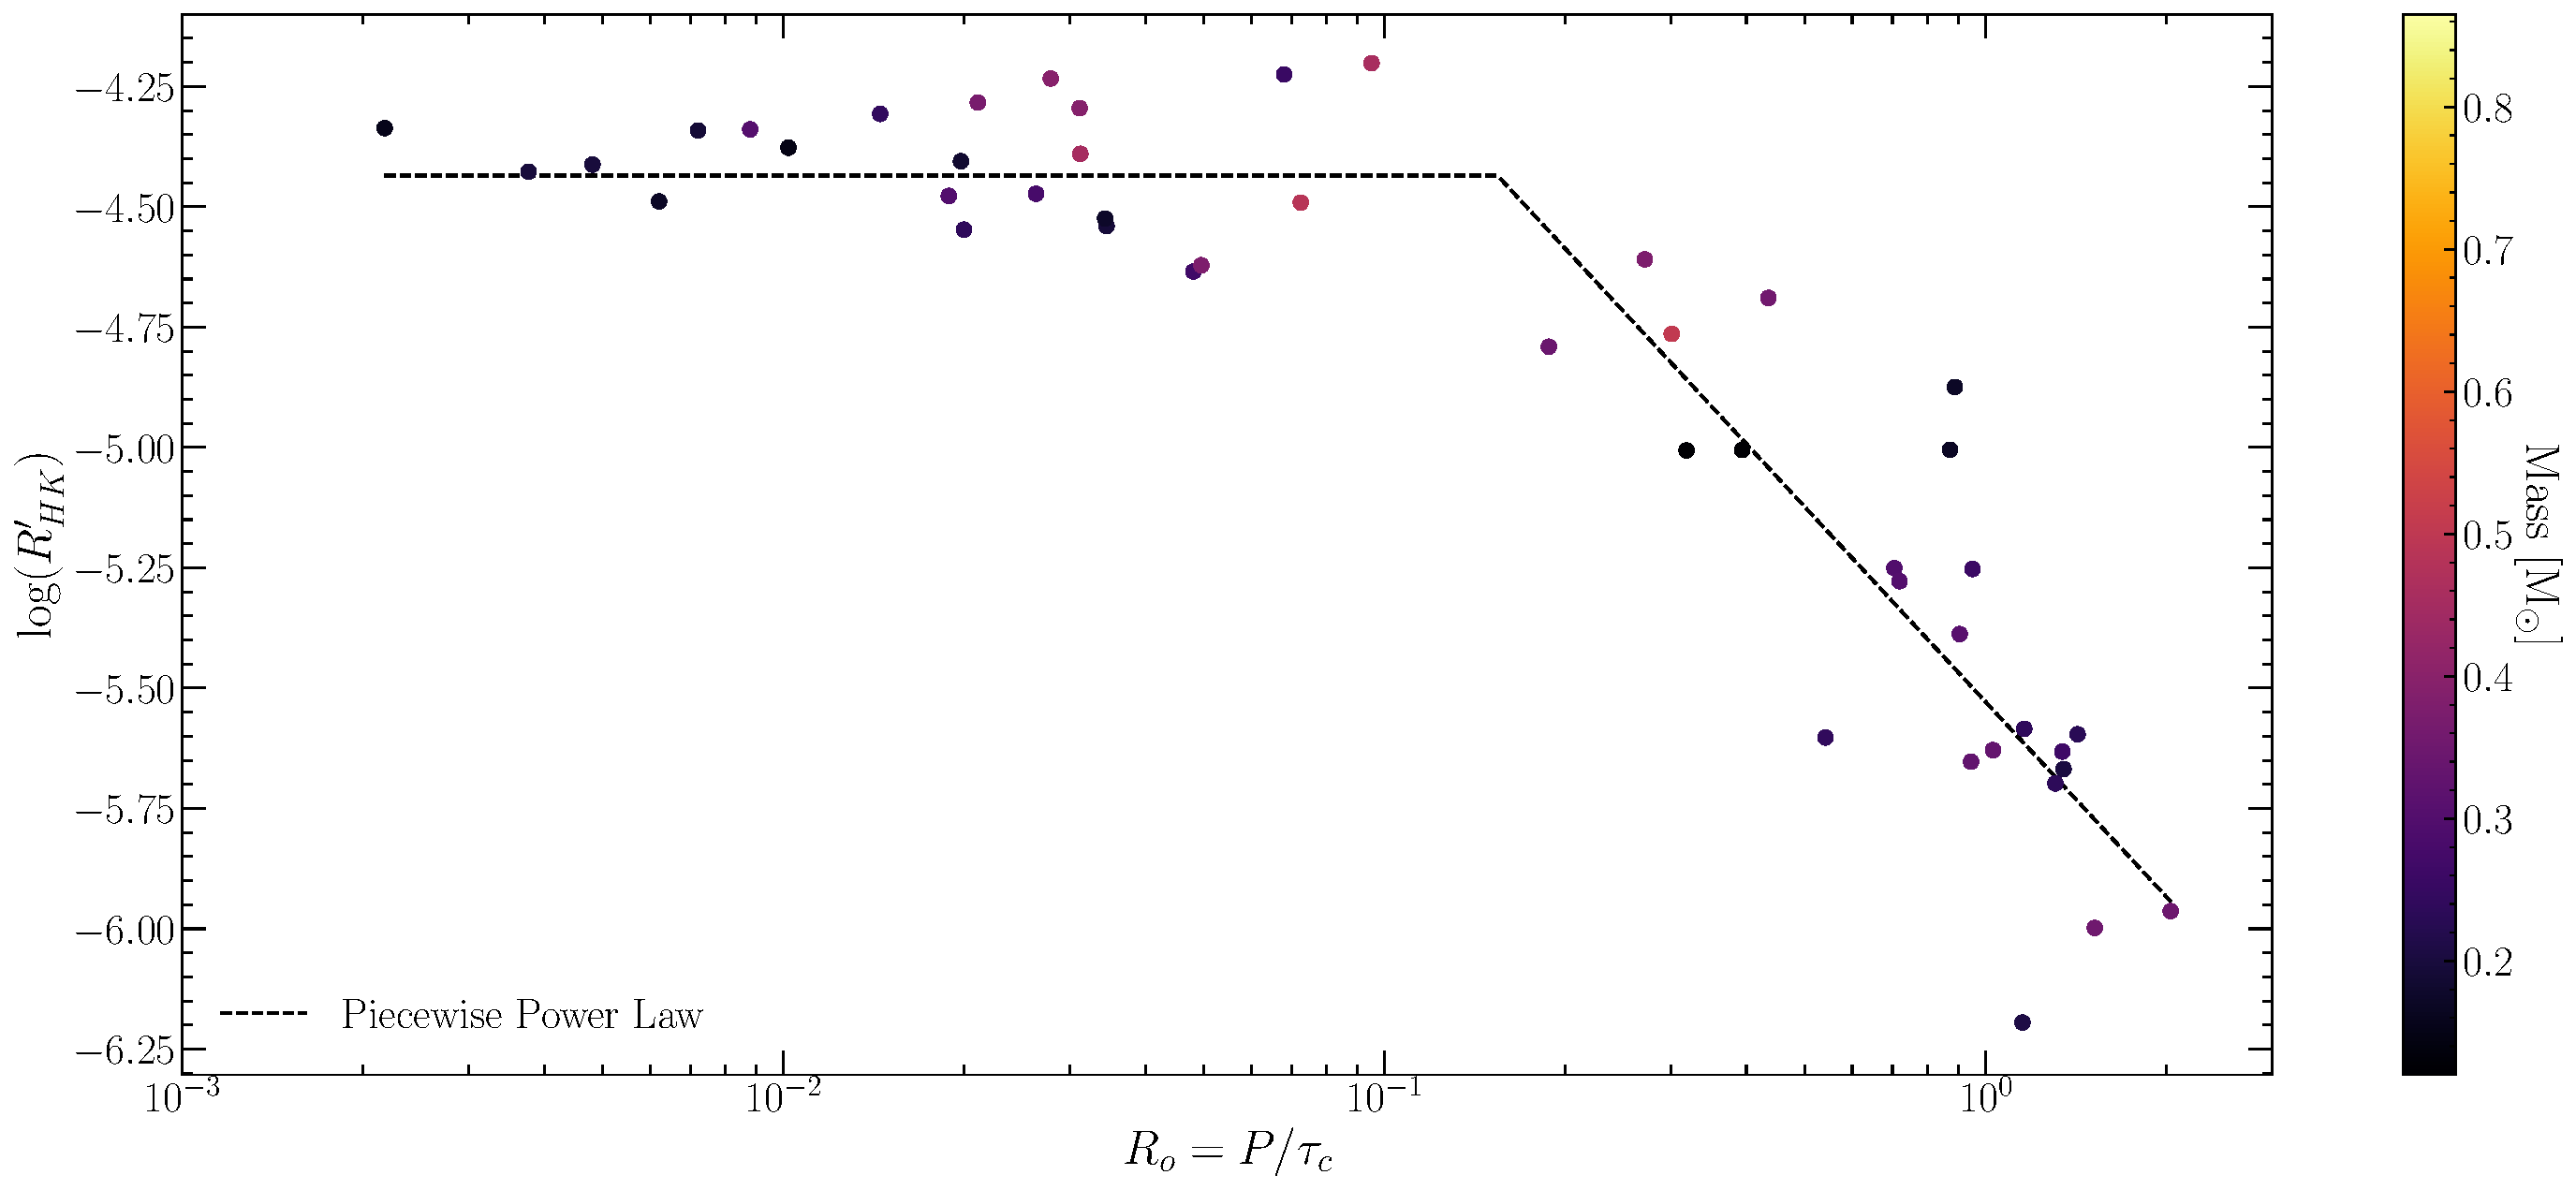
\includegraphics[width=0.9\textwidth]{figures/magActivity/RpHKvsR0_MC_justThisPaper.pdf}
	\caption{Rotation activity relation from this work. The color axis gives
	each stars mass. The dashed line is the best fit to our data set.}
    \label{fig:RpHKvsRossbySelf}
\end{figure*}
\begin{figure*}
    \centering
    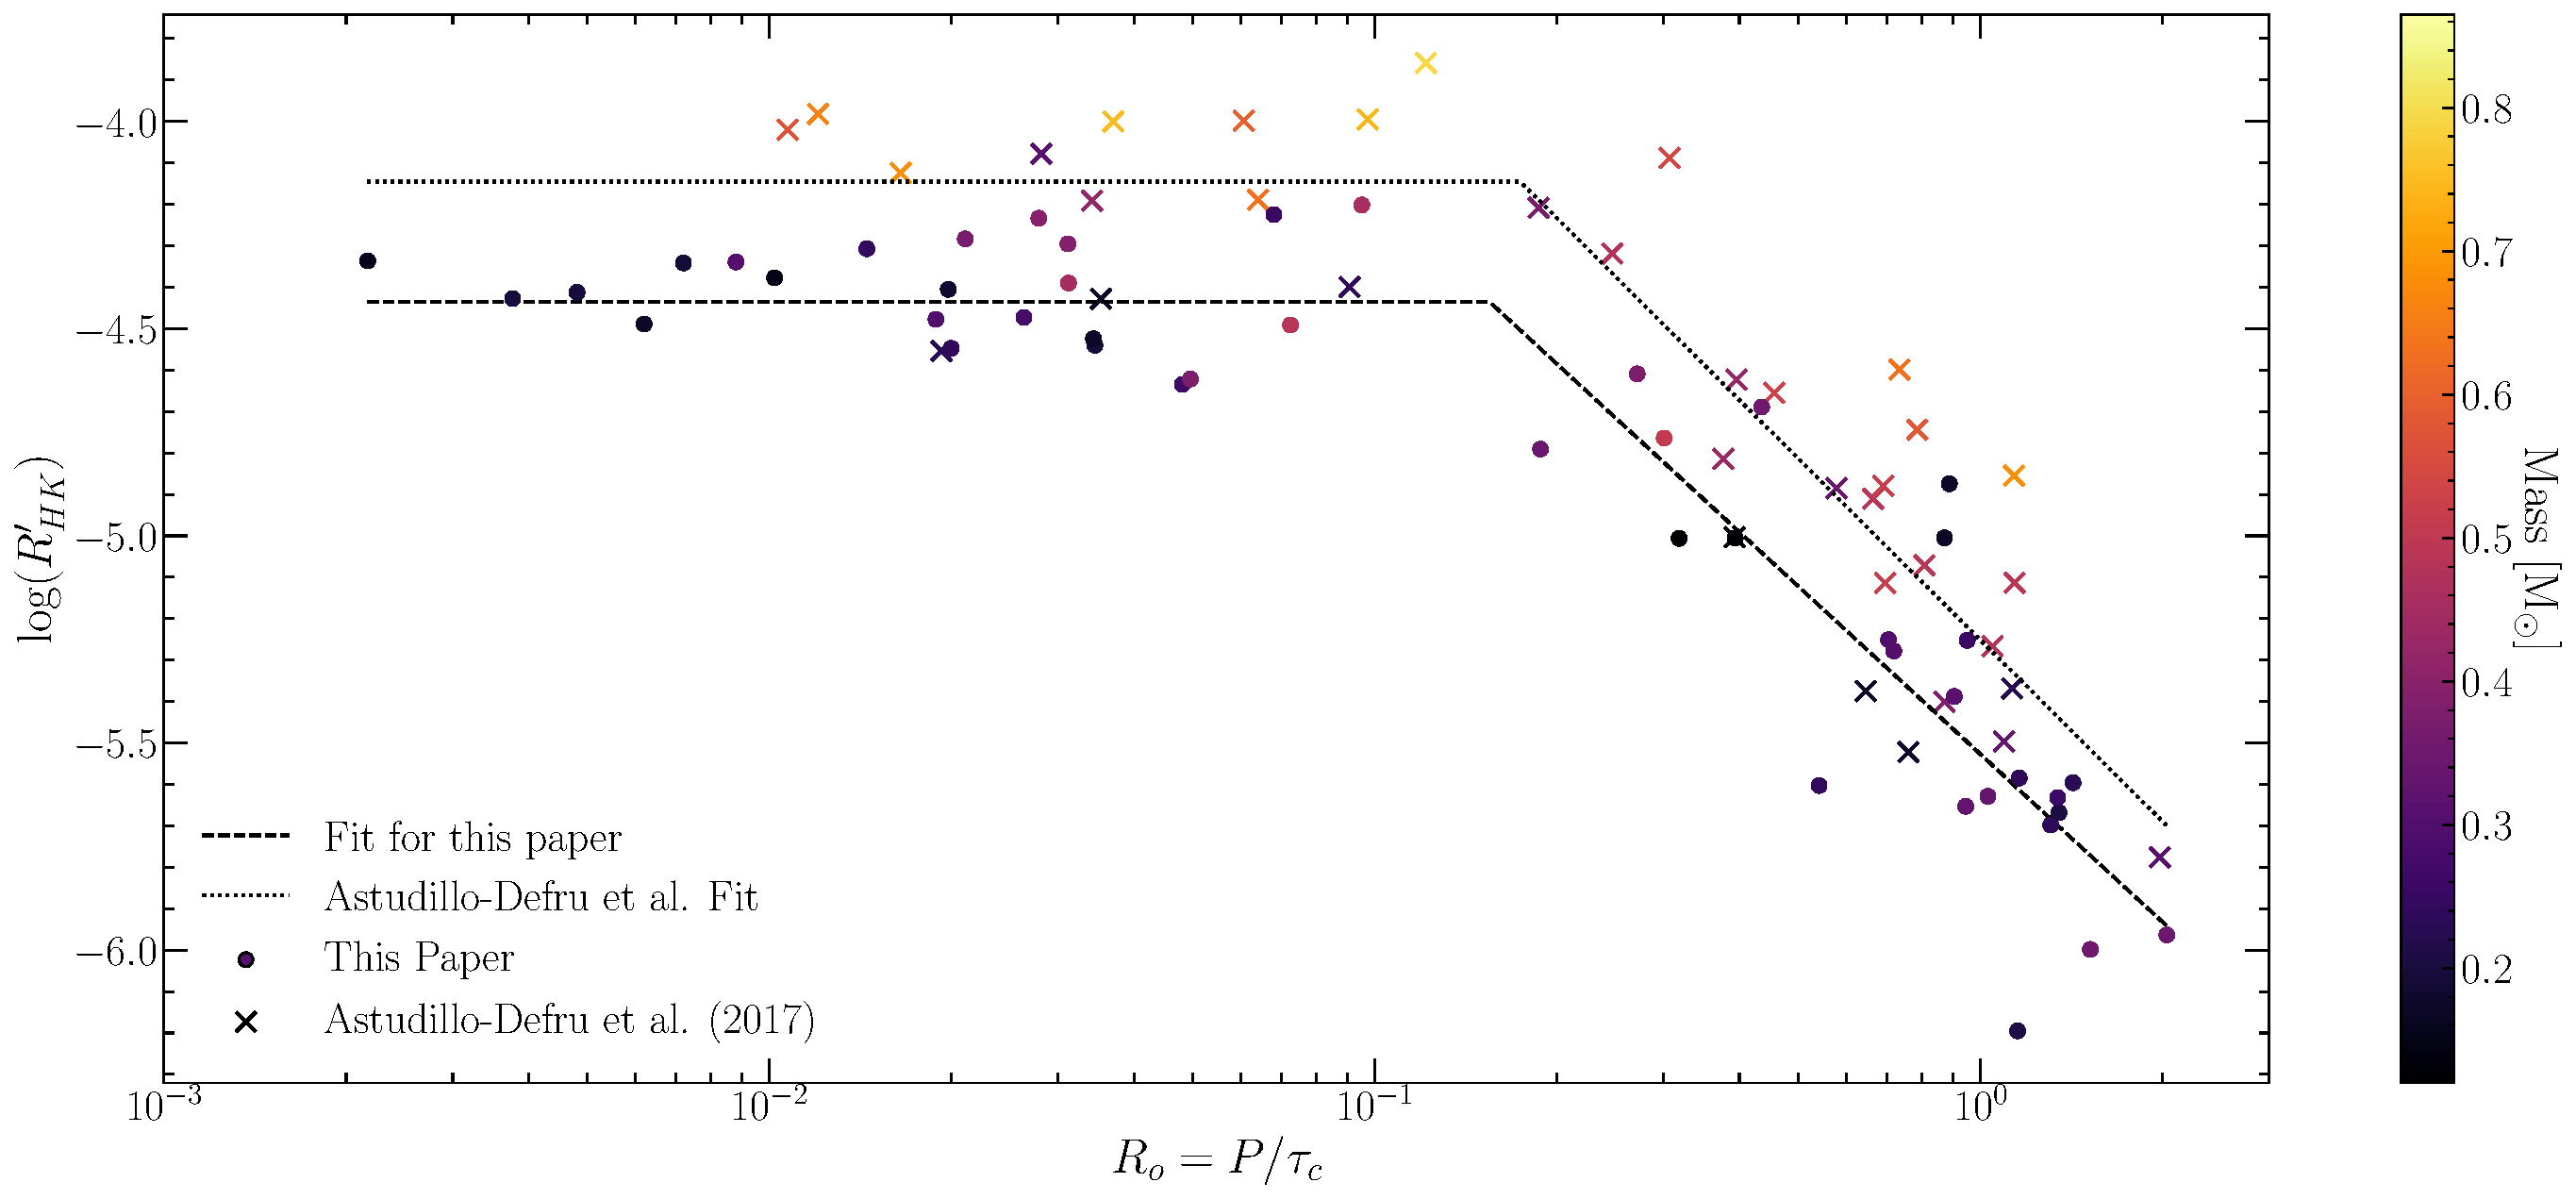
\includegraphics[width=0.9\textwidth]{figures/magActivity/RpHKvsR0_MC.pdf}
	\caption{Rotation activity relation for both our work and \citet{Def17}.
	The dotted line is the best fit to the re-derived rotation-activity
	relation from \citet{Def17}.  Note that targets from \citet{Def17} are
	systematically higher than targets presented here as a consequence of the
	range in mass probed by the samples.}
    \label{fig:RpHKvsRossbyDef}
\end{figure*}
\begin{figure*}
    \centering
    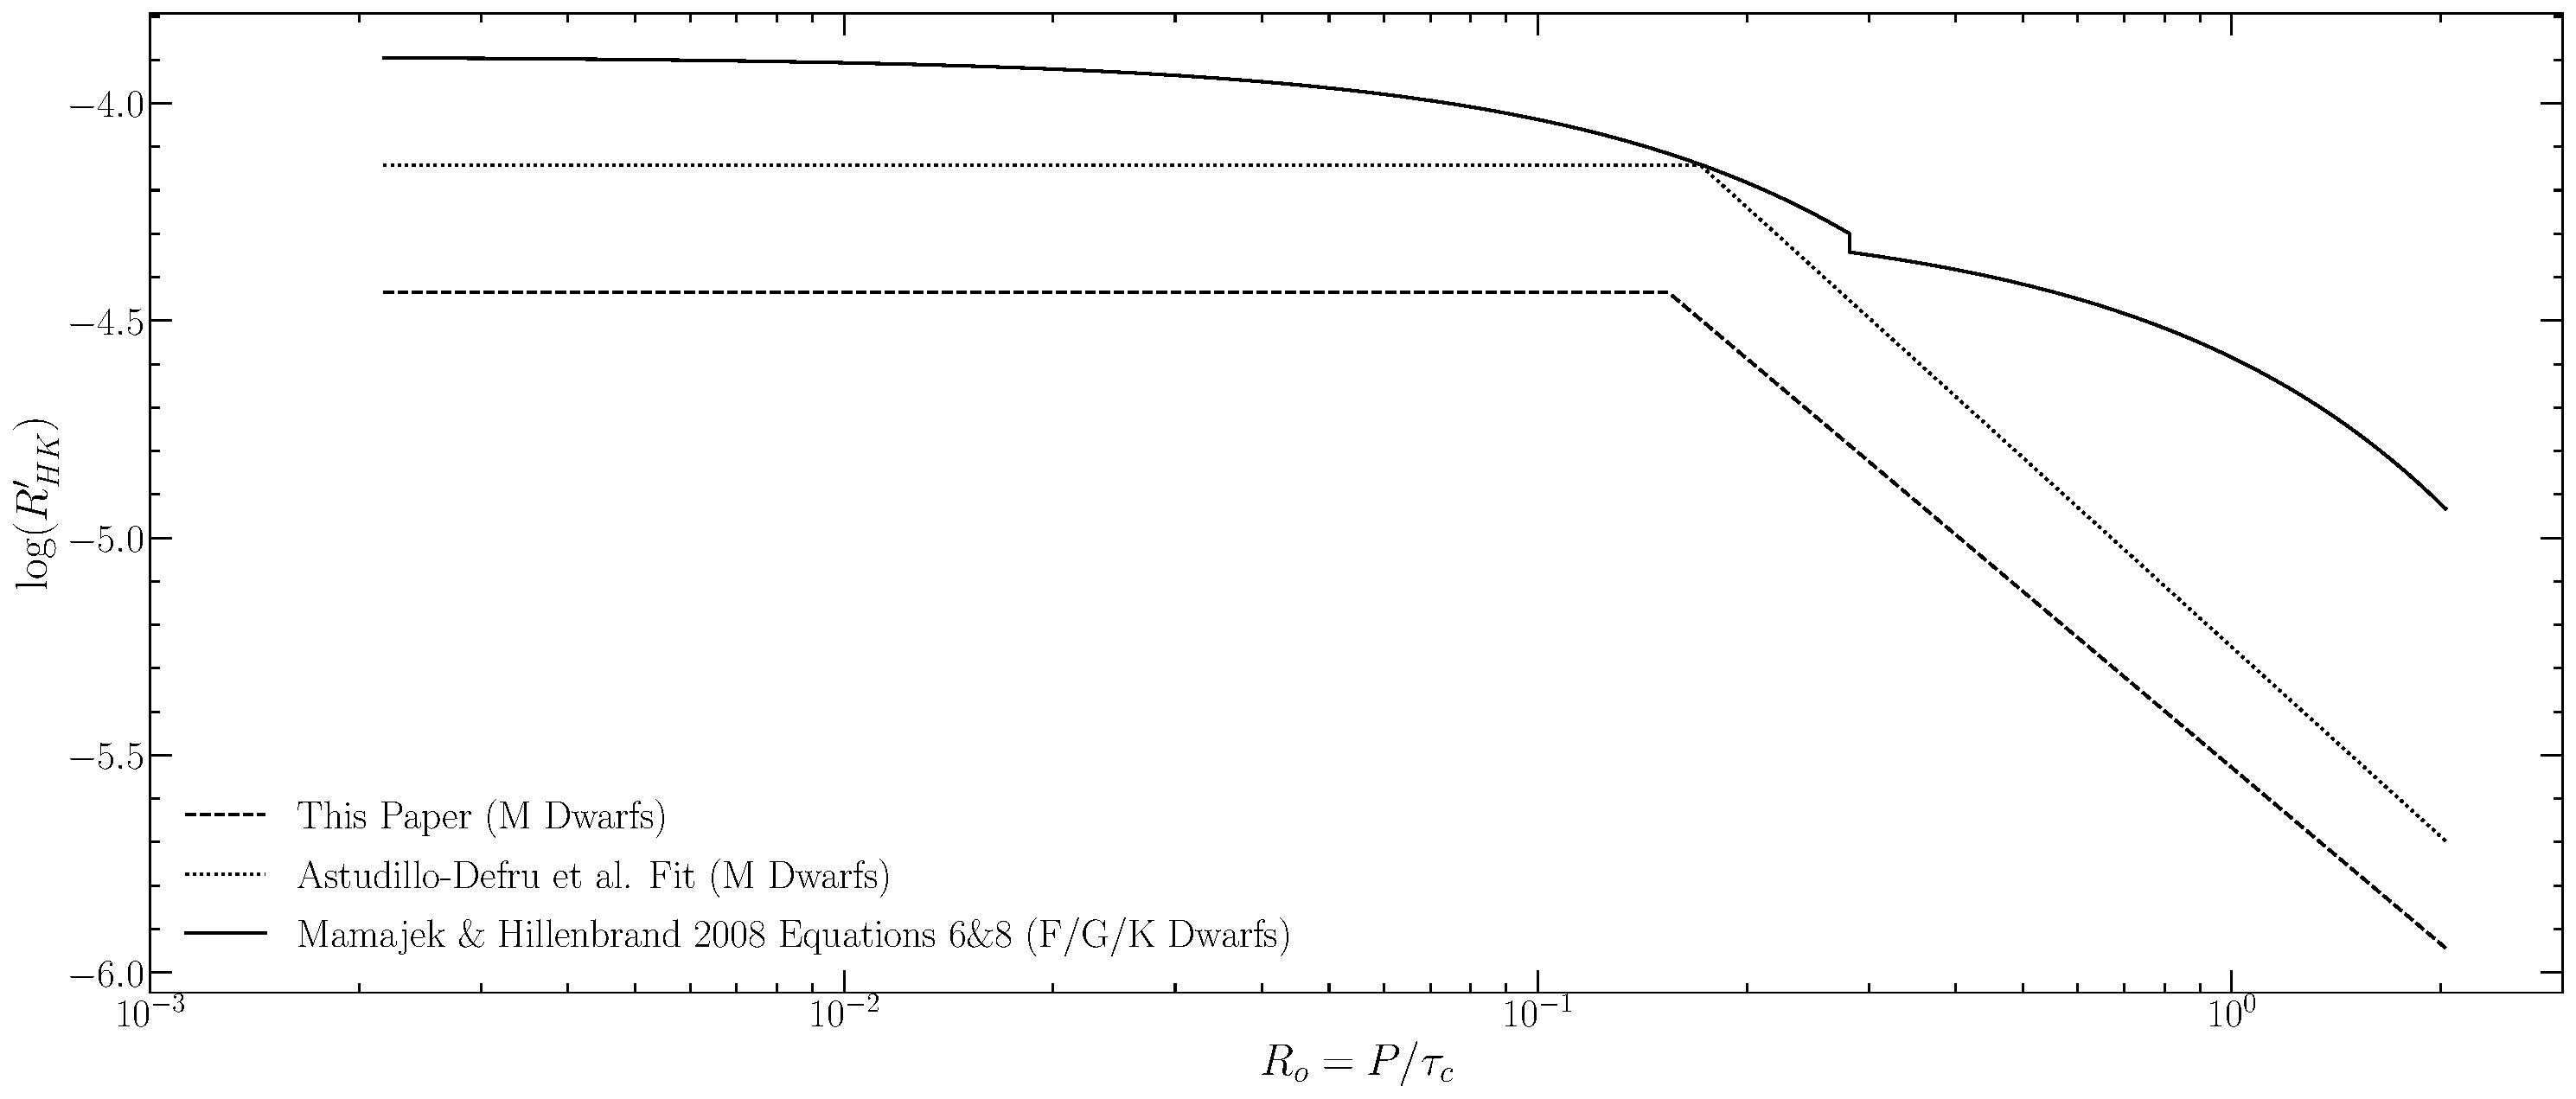
\includegraphics[width=0.9\textwidth]{figures/magActivity/RpHKvsR0_MC_fits.pdf}
	\caption{Derived rotation-activity curves from this work, \citet{Def17} and
	\citet{Mamajek2008}. Note both that \citet{Mamajek2008} focuses their work
	on earlier spectral classes and fits the rotation activity relation in
	linear space.}
    \label{fig:RpHKvsRossbyFits}
\end{figure*}

We find best fit parameters with one $\sigma$ errors:
\begin{itemize}
    \item $k = -1.347\pm 0.203$
    \item $Ro_{s} =  0.155\pm0.045$
    \item $\log(R_{s}) = -4.436\pm0.048$

\end{itemize}
A comparison of the rotation activity derived in this work to those
from both \citet{Def17} and \citet{Mamajek2008} is presented in Figure
\ref{fig:RpHKvsRossbyFits}. For the 6 targets which do not have measured
rotational periods we include an estimate of $Ro$ and $p_{rot}$ in the machine
readable version of Table \ref{tab:finalData}. The convective overturn
timescale for one of these 6 targets (2MASS J13464102-5830117) can not be
inferred via Equation \ref{eqn:convectiveOverturn} as it lacks a V-K color
measurement. Instead, we infer $\tau_{c}$ via \citet{Wri18} Equation 6 (this
paper Equation \ref{eqn:ConvectiveOverturnTimeMass}) using mass. Similar to our
manner of inferring $\tau_{c}$ via color, when inferring $\tau_c$ via mass, we
adopt the larger of the two antisymmetric errors from \citet{Wri18}.

\begin{equation}\label{eqn:ConvectiveOverturnTimeMass}
	\log_{10}(\tau_{c}) = 2.33\pm0.06 - 1.5\pm0.21\left(M/M_{\odot}\right) + 0.31\pm0.17\left(M/M_{\odot}\right)^{2}
\end{equation}

Note that $R'_{HK}$ for one of six of these targets (2MASS
J15165576-0037116) is consistent to within 1$\sigma$ of the saturated value;
therefore, the reported $Ro$ for this target should only be taken as an upper
bound. The remaining five targets have measured $R'_{HK}$ values consistent
with the unsaturated regime. Estimated periods are consistent with previous
constraints. Of the six stars, two were listed as non-detections in
\citet{Newton2018}, and the remaining four as uncertain (possible) detections.
Of the four classed as uncertain, 2MASS 12384914-3822527 and 2MASS
19204795-4533283 have candidate periods $>100$ days and non-detections of
H-alpha emission \citep{Hawley96}. These two stars and the two non-detections
have Ca II H\&K activity levels suggesting very long periods. 2MASS
13464102-5830117 has a candidate period of 45 days, and 2MASS 15165576-0037116
of 0.8 days, both consistent with their higher levels of Ca II H\&K emission.

As a test of the proposed weak correlation between activity and rotation in the
``saturated'' regime seen in some works \citep{Mamajek2008,
Reiners2014, Leh20, Med20} --- though not in others \citep{Wri11, Nunez2015,
Newton2017} ---   we fit a second model whose power law index is allowed to
vary at $Ro < Ro_{s}$. We find a saturated regime power law index of
$-0.052\pm0.117$, consistent with 0 to within 1$\sigma$. Moreover,
all other parameter for this model are consistent to within one $\sigma$ of the
nominal  parameters for the model where the index is constrained to 0 below
$Ro=Ro_{s}$. We can constrain the slope in the saturated
regime to be between -0.363 and 0.259 at the $3\sigma$ confidence level.
Ultimately, we adopt the most standard activity interpretation, a
fully-saturated regime at $Ro < Ro_{s}$. 

We investigate whether our lack of detection of a slope for $Ro <
Ro_{s}$ is due to the limited number of observations in that region when
compared to other works \citep[e.g.][93 targets $Ro < Ro_{s}$]{Med20} through
injection and recovery tests. We inject, fake, rotation-activity measurements
into the saturated regime with an a priori slope of -0.13 --- the same as in
\citeauthor{Med20}. These fake data are given a standard deviation equal to the
standard deviation of our residuals ($12\%$). We perform the same MCMC model
fitting to this new data set as was done with the original data set multiple
times, each with progressively more injected data, until we can detect the
injected slope to the three sigma confidence level. Ultimately, we need more
than 65 data points --- 43 more than we observed in the saturated regime --- to
consistently recover this slope. Therefore, given the spread of our data we
cannot detect slopes on the order of what has previously been reported in the
literature.

We observe a gap in rotational period over a comparable range to the
one presented in \citet{Newton2016} Figure 2. Namely, that M-dwarfs are
preferentially observed as either fast or slow rotators, with a seeming lack of
stars existing at mid rotational periods. This period gap manifests in the
Rossby Number and can be seen in Figure \ref{fig:RpHKvsRossbyDef} as a lack of
our targets near to the knee-point in the fit. This period gap likely
corresponds to that seen by \citet{Browning2010}, who found a paucity of M
dwarfs at intermediate activity levels in Ca II H\&K and note the similarity to
the Vaughn-Preston gap established in higher mass stars \citep{vaughan1980}.
\citet{Magaudda2020} also identify a double-gap in x-ray activity for stars in
the unsaturated regime; it is not clear that the gap we see is related. As a
consequence of this period gap, there exists a degeneracy in our data
between moving the knee-point and allowing the activity level to vary in the
saturated regime.  In the following, we adopt the model of a fully saturated
regime.

We wish to compare our best fit parameters to those derived in \citet{Def17};
however, the authors of that paper do not fit the knee-point of the
rotation-activity relation. They select the canonical value for the rotational
period separating the saturated regime from the unsaturated regime ($P_{rot,s}
= 10$ days) and use a fixed convective overturn timescale ($\tau_{c} = 70$
days). To make our comparison more meaningful we use the $P_{rot}$ and $V-K$
colors presented in \citet{Def17} to re-derive $Ro$ values using $\tau_{c}$
\citep{Wri18}. Doing this for all targets presented in \citet{Def17} Table 3
and fitting the same piecewise power law as before, we find best fit parameters
of $Ro_{s} = 0.17\pm0.04$, $\log(R_{s}) = -4.140\pm0.067$, and
$k=-1.43\pm0.21$. Compared to the best fit parameters for our data, $Ro_{s}$
and the unsaturated regime's index, $k$, are consistent to within one sigma,
while the saturated value, $R_{s}$, differs. 

The mass ranges of our respective samples explain the differences in saturation
values between our work and that of \citet{Def17}. Our work focuses on
mid-to-late M-dwarfs and includes no stars above a mass of $0.5$ M$_{\odot}$
(Figure \ref{fig:massDistribution}).  The strength of Ca II H\&K
emission is known to decrease as stellar mass decreases \citep{Schrijver1987,
Rauscher2006, Hou17}. As \citet{Rauscher2006} note, this is the opposite as the
trend seen in H-alpha; the latter primarily reflects the increasing length of
time that lower M dwarfs remain active and rapidly rotating \citep{West2015,
Newton2016}.

A mass dependence can be seen in Figure 10 in \citet{Def17}, consistent
with expectations from the literature. If we clip the data from \citet{Def17}
Table 3 to the same mass range as our data-set ($M_{*} < 0.5M_{\odot}$) and fit
the same function as above, we find that all best fit parameters are consistent
to within one sigma between the two data-sets. 

\begin{figure}
    \centering
    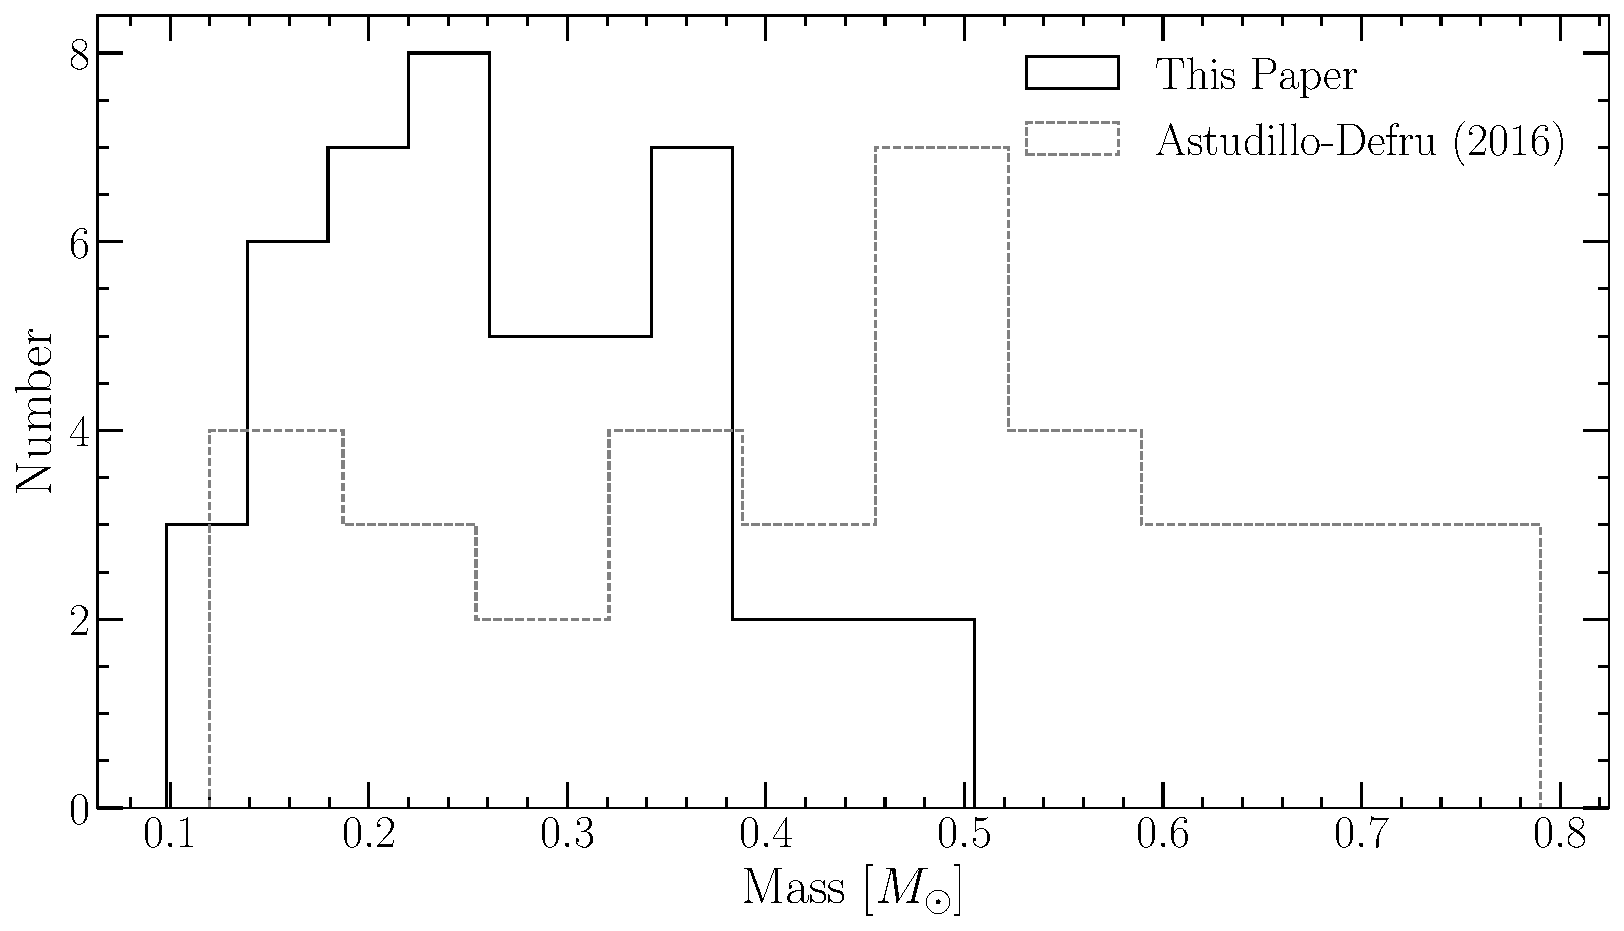
\includegraphics[width=0.85\textwidth]{figures/magActivity/B2020vsAD2016_Masses.pdf}
	\caption{Distribution of masses between our sample and the sample presented
	in \citet{Def17}. Note how the two studies have approximately the same
	sample sizes; however, our sample is more tightly concentrated at lower
	masses \textbackslash later spectral classes.}
    \label{fig:massDistribution}
\end{figure}

We also compare our best fit $Ro_{s}$ to both those derived in
\citet{Newton2017} using $H_{\alpha}$ as an activity measure and those derived
in \citep{ Wri18, Magaudda2020} using $L_{X}/L_{bol}$ as an activity measure.
Works using $L_{X}/L_{bol}$ identify a similar, yet not consistent to within
one sigma result for $Ro_{s}$; while, the value of $k$ we find here is
consistent between all four works. Therefore, we find similar results not only
to other work using the same activity tracer, but also a power-law slope that
is consistent with work using different tracers. 


\section{Conclusion}\label{sec:conclusion}
%
% \begin{figure}[H]
% 	\centering
% 	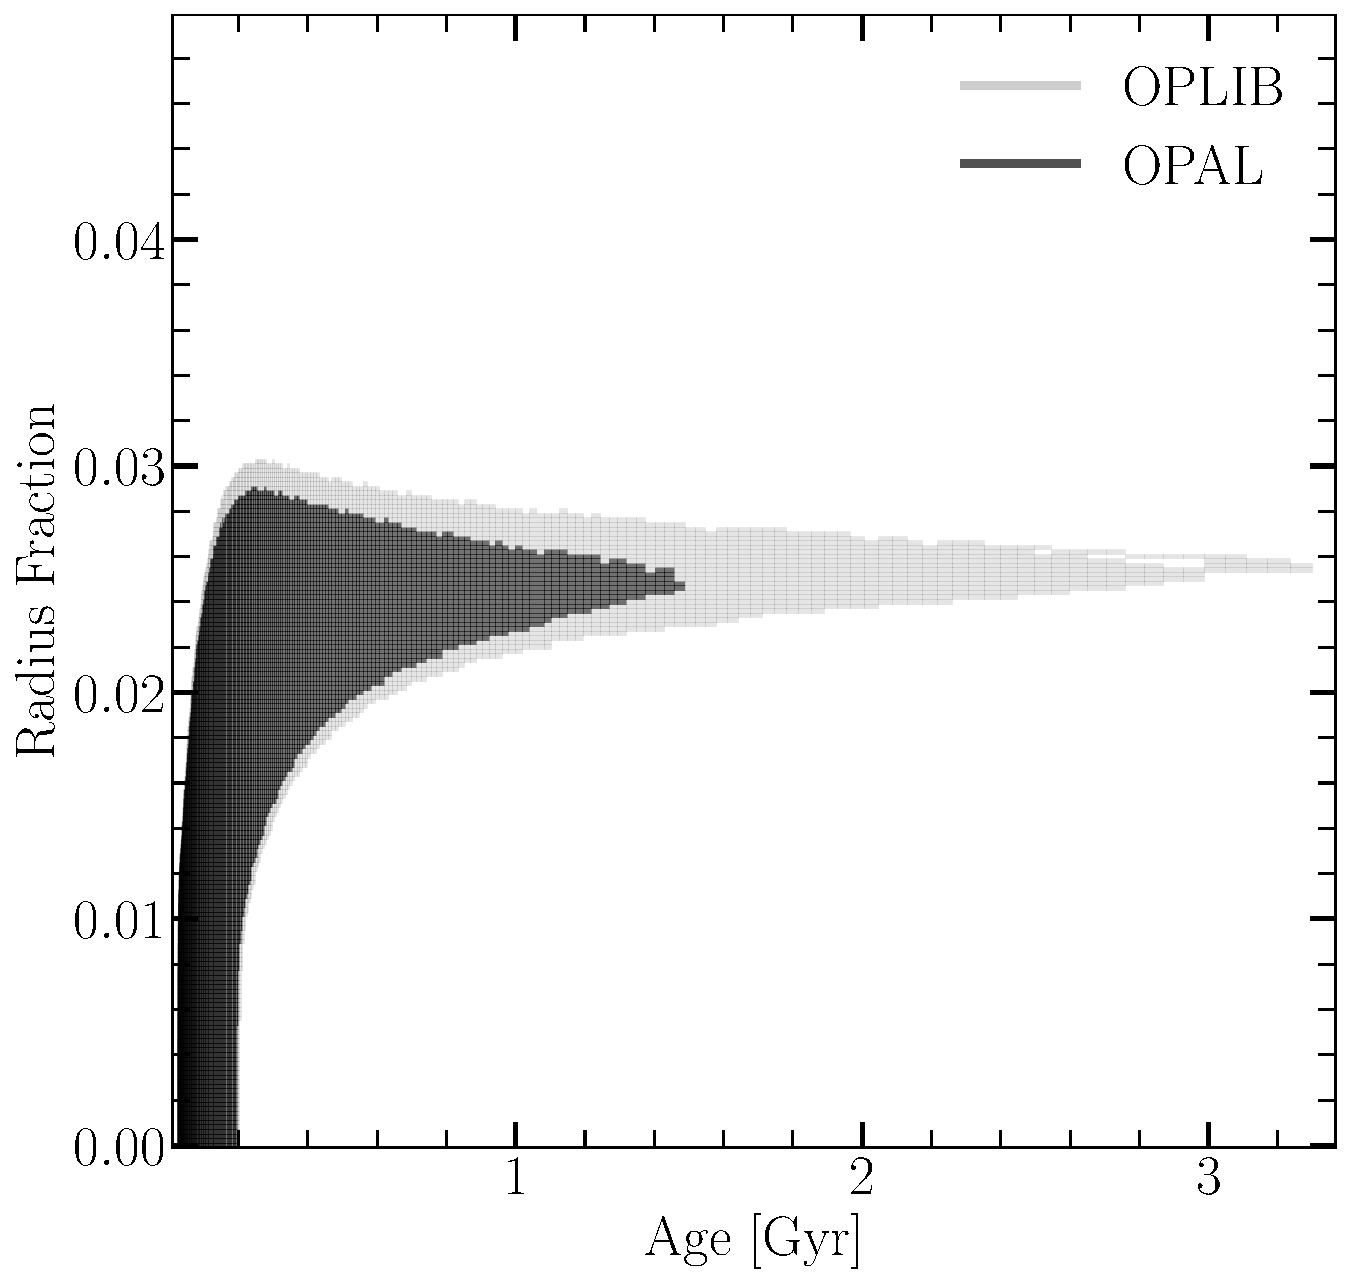
\includegraphics[width=0.85\textwidth]{figures/jaoOpacity/SameMassConvectiveZoneComp.pdf}
% 	\caption{Portions of 0.3526 $M_{\odot}$ OPAL and OPLIB stellar models
% 	showing the interior shells which are radiative (black region). Note that
% 	for clarity only one convective mixing event from each model is shown. Note
% 	how the radiative zone in the OPLIB model is larger.}
% 	\label{fig:Unstable}
% \end{figure}
%
% \begin{figure}[H]
% 	\centering
% 	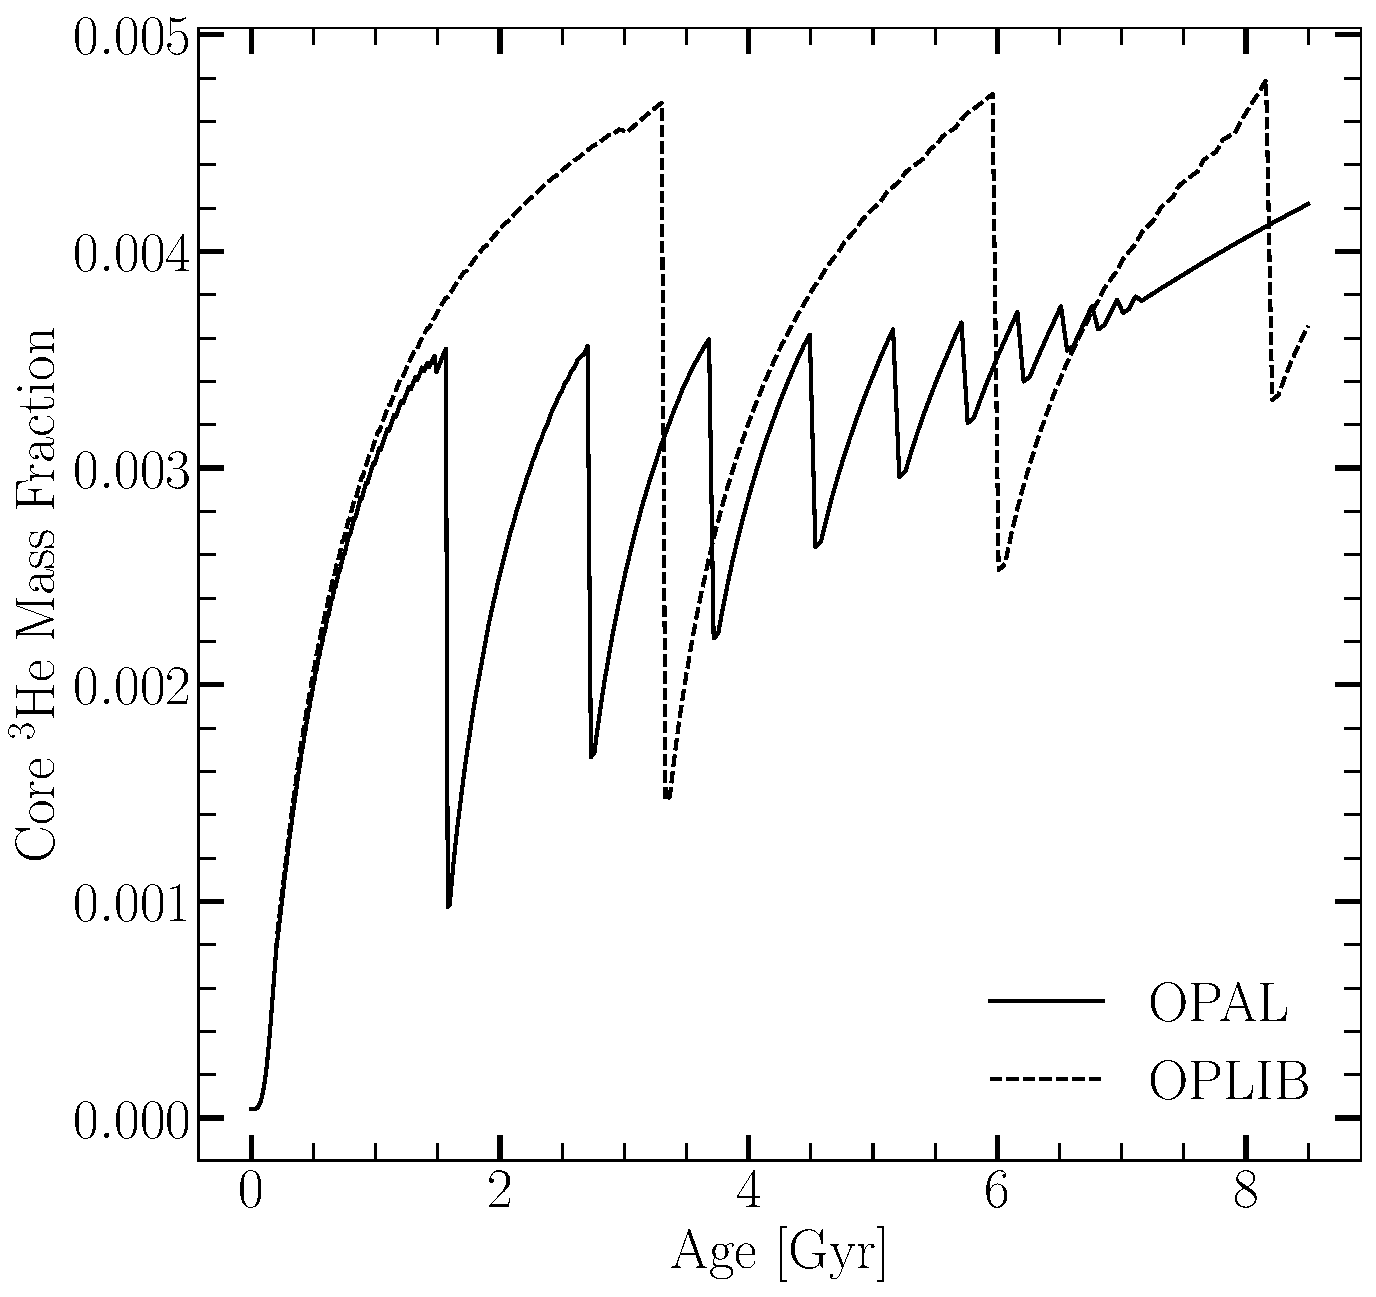
\includegraphics[width=0.85\textwidth]{figures/jaoOpacity/Core3HECompSameMass.pdf}
% 	\caption{Core $^{3}$He mass fraction for  0.3526 $M_{\odot}$ models evolved
% 	with OPAL and OPLIB (within the Jao Gap's mass range for both). Note how
% 	the OPLIB model's core $^{3}$He mass fraction grows at approximately the
% 	same rate as the OPAL model's but continues uninterrupted for longer.}
% 	\label{fig:OPALOPLIB3He}
% \end{figure}
The Jao Gap provides an intriguing probe into the interior physics of M Dwarfs
stars where traditional methods of studying interiors break down. However,
before detailed physics may be inferred it is essential to have models which
are well matched to observations. Here we investigate whether the OPLIB opacity
tables reproduce the Jao Gap location and structure more accurately than the
widely used OPAL opacity tables. We find that while the OPLIB tables do shift
the Jao Gap location more in line with observations, by approximately 0.05
magnitudes, the shift is small enough that it is likely not distinguishable
from noise due to population age and chemical variation. However, future
measurement of [Fe/H] for stars within the gap will be helpful in constraining
the degree to which the gap should be smeared by these theoretical models.

We also find that both the color and magnitude of the Jao Gap are
correlated to the convective mixing length parameter. Specifically, a lower
mixing length parameter will bring the gap in the populations presented in this
paper more in line with the current best estimate for the actual gap magnitude.
Using this relation it may be possible for mixing length to be calibrated for
low mass stars such that models match the Jao Gap location. Further, the Jao
gap location may provide a test of alternative convection models such as
entropy calibrated convection \citep{Spada2021}. Both of these potential uses
require careful handling of other uncertanties such as the uncertanties in
bolometric correction, population composition, and population age. As we
currently do not have reason to suspect that the mixing length for the low mass
stars in the DR2 and ERD3 CMD is substantially lower than that of the sun we
leave the investigation of these potential additional uses for future work.

Finally, we do not find that the OPLIB opacity tables help in reproducing the
as yet unexplained wedge shape of the observed Gap.




\acknowledgments{
	This work has made use of the NASA astrophysical data system (ADS). We
	would like to thank Elisabeth Newton, Aaron Dotter, and Gregory Feiden for
	their support and for useful discussion related to the topic of this paper.
	We would like to thank our reviewer for their critical eye and their
	guidance to investigate to effects of the mixing length on the Gap
	Location. Additionally, we would like to thank James Colgan and the Los
	Alamos T-1 group for their assistance with the OPLIB opacity tables and
	support for the public release of \texttt{pyTOPSScrape}. We acknowledge the
	support of a NASA grant (No. 80NSSC18K0634). 
}
\acknowledgments

% \begin{acknowledgments}
% 	This work has made use of the NASA astrophysical data system (ADS). We
% 	would like to thank Elisabeth Newton, Aaron Dotter, and Gregory Feiden for
% 	their support and for useful discussion related to the topic of this paper.
% 	We would like to thank our reviewer for their critical eye and their
% 	guidance to investigate to effects of the mixing length on the Gap
% 	Location. Additionally, we would like to thank James Colgan and the Los
% 	Alamos T-1 group for their assistance with the OPLIB opacity tables and
% 	support for the public release of \texttt{pyTOPSScrape}. We acknowledge the
% 	support of a NASA grant (No. 80NSSC18K0634). 
% \end{acknowledgments}

\software{
	The Dartmouth Stellar Evolution Program (DSEP) \citep{Dotter2008},
	\texttt{BeautifulSoup} \citep{richardson2007beautiful},
	\texttt{mechanize} \citep{chandra2015python},
	\texttt{FreeEOS} \citep{Irwin2012},
	\texttt{pyTOPSScrape} \citep{Boudreaux22}
}

\appendix

\section{\texttt{pyTOPSScrape}}\label{apx:pytopsscrape}
\texttt{pyTOPSScrape} provides an easy to use command line and python interface
for the OPLIB opacity tables accessed through the TOPS web form. Extensive
documentation of both the command line and programmatic interfaces is linked
in the version controlled repository. However, here we provide a brief,
illustrative, example of potential use.

Assuming \texttt{pyTOPSScrape} has been installed and given some working
directory which contains a file describing a base composition (``comp.dat'')
and another file containing a list of rescalings of that base composition
(``rescalings.dat'') (both of these file formats are described in detail in the
documentation), one can query OPLIB opacity tables and convert them to a form
mimicking that of type 1 OPAL high temperature opacity tables using the
following shell command.

{\small
\begin{verbatim}
	$ generateTOPStables comp.dat rescalings.dat -d ./TOPSCache -o out.opac -j 20
\end{verbatim}
}

\noindent For further examples of pyTOPSScrape please visit the repository.


\section{Interpolating $\rho \rightarrow $ R}\label{apx:interp}
OPLIB parameterizes $\kappa_{R}$ as a function of mass density, temperature in keV,
and composition. Type 1 OPAL high temperature opacity tables, which DSEP and
many other stellar evolution programs use, instead parameterizes opacity as a function
of temperature in Kelvin, $R$ (Equation \ref{eqn:Req}), and composition. The
conversion from temperature in keV to Kelvin is trivial (Equation
\ref{eqn:K2Kev}).
\begin{align}\label{eqn:Req}
	R = \frac{\rho}{T_{6}^{3}}
\end{align}
\begin{align}\label{eqn:K2Kev}
	T_{K} = T_{keV} * 11604525.0061657
\end{align}
However, the conversion from mass density to $R$ is more involved. Because $R$
is coupled with both mass density and temperature there there is no way to
directly convert tabulated values of opacity reported in the OPLIB tables to
their equivalents in $R$ space. The TOPS webform does allow for a
density range to be specified at a specific temperature, which allows for R
values to be directly specified. However, issuing a query to the TOPS webform
for not just every composition in a Type 1 OPAL high temperature opacity table
but also every temperature for every composition will increase the number of
calls to the webform by a factor of 70. Therefore, instead of directly
specifying R through the density range we choose to query tables over a
broad temperature and density range and then rotate these tables,
interpolating $\kappa_{R}(\rho,T_{eff}) \rightarrow \kappa_{R}(R,T_{eff})$. 


To perform this rotation we use the \texttt{interp2d} function within
\texttt{scipy}'s \texttt{interpolate} \citep{2020SciPy-NMeth} module to
construct a cubic bivariate B-spline \citep{Dierckx1981} interpolating function
$s$, with a smoothing factor of 0, representing the surface $\kappa_{R}(\rho,
T_{eff})$. For each $R^{i}$ and $T^{j}_{eff}$ reported in type 1 OPAL tables,
we evaluate Equation \ref{eqn:Req} to find $\rho^{ij} =
\rho(T^{j}_{eff},R^{i})$.  Opacities in $T_{eff}$, $R$ space are then inferred
as $\kappa^{ij}_{R}(R^{i},T^{j}_{eff}) = s(\rho^{ij}, T^{j}_{eff})$. 

As first-order validation of this interpolation scheme we can perform a similar
interpolation in the opposite direction, rotating the tables back to
$\kappa_{R}(\rho, T_{eff})$ and then comparing the initial, ``raw'', opacities
to those which have gone through the interpolations process. Figure
\ref{fig:fracdiff} shows the fractional difference between the raw opacities
and a set which have gone through this double interpolation. The red line
denotes $\log(R)=-0.79$ where models near the Jao Gap mass range will
tend to sit for much of their radius. Along the $\log(R)=-0.79$ line the mean
fractional difference is $\langle \delta \rangle = 0.005$ with an uncertainty of
$\sigma_{\langle\delta\rangle} = 0.013$. One point of note is that, because the
initial rotation into $\log(R)$ space also reduces the domain of the opacity
function, interpolation-edge effects which we avoid initially by extending the
domain past what type 1 OPAL tables include cannot be avoided when
interpolating back into $\rho$ space. 

\begin{figure}
	\centering
	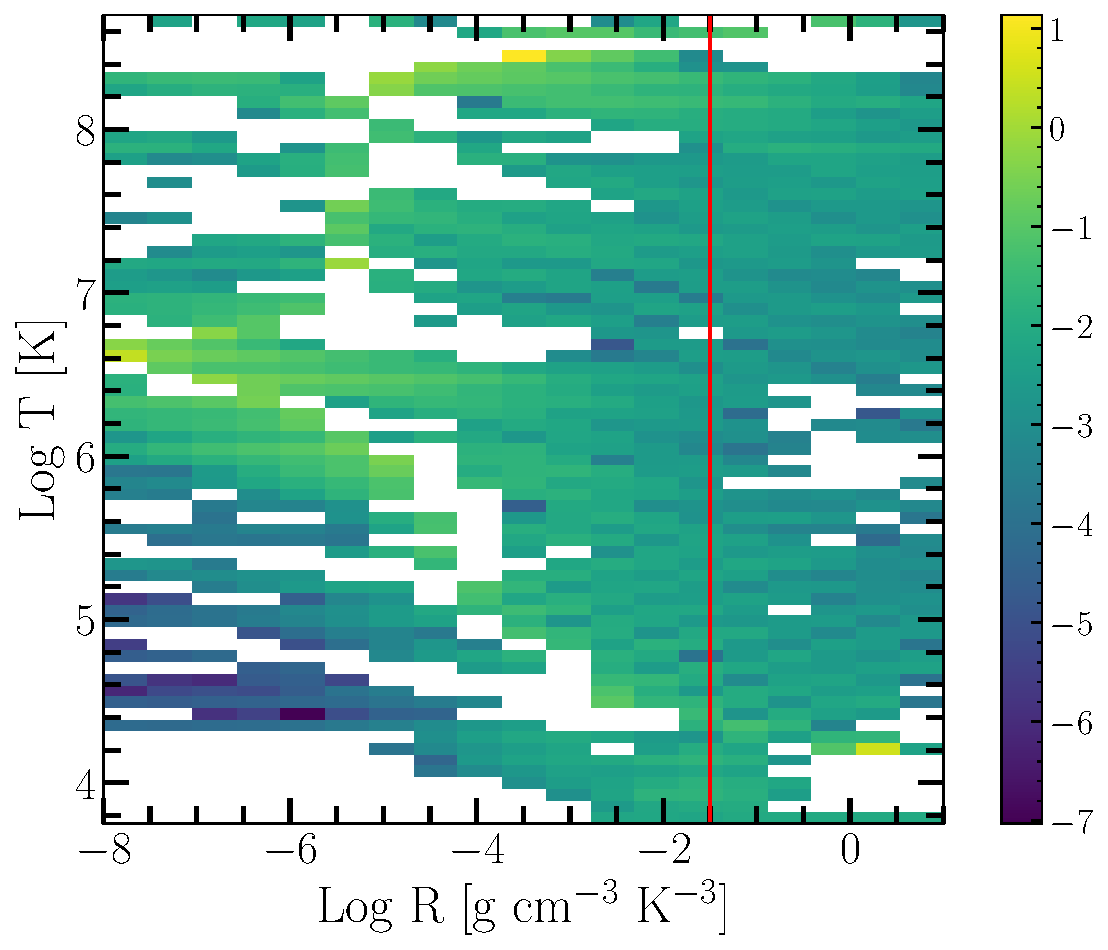
\includegraphics[width=0.85\textwidth]{figures/jaoOpacity/FractionalDifference.pdf}
	\caption{Log Fractional Difference between opacities in $\kappa_{R}(\rho,
	T_{eff})$ space directly queried from the OPLIB web-form and those which
	have been interpolated into $\log(R)$ space and back. Note that, due to the
	temperature grid of type 1 OPAL tables not aligning perfectly which the temperature
	grid OPLIB uses there may be edge effects where the interpolation is poorly
	constrained. The red line corresponds to $\log(R) = -0.79$ where much of a
	stellar model's radius exists.}
	\label{fig:fracdiff}
\end{figure}





\bibliography{ms}{}
\bibliographystyle{aasjournal}


\end{document}

